%\documentclass{IEEEtran}
\documentclass{article}
\usepackage[T1]{fontenc}
\usepackage{csquotes}
\usepackage{amsfonts,amsmath,amssymb,amsthm}
%\usepackage{setspace}
\usepackage{xspace}%,enumitem}
%\usepackage{times}
\usepackage{fullpage}
%\usepackage{hyperref}
%\doublespacing
\usepackage{color}
\usepackage{numdef}
\let\labelindent\relax
\usepackage[shortlabels]{enumitem}
\usepackage{amsopn}
\usepackage{multirow}
\usepackage{framed}
%\usepackage{hyperref} 
\usepackage{graphicx}
\usepackage{cite}
\usepackage{adjustbox}

\usepackage{dsfont}
\usepackage{cleveref}
\usepackage{tikz}
\usepackage{url}
\usepackage{algpseudocode,algorithm,algorithmicx}
\providecommand{\sqbinom}{\genfrac{\lbrack}{\rbrack}{0pt}{}}
\DeclareMathOperator{\spn}{span}

\author{
   Sean Bowe
  \texttt{sean@z.cash}
  \and
  Ariel Gabizon 
  \texttt{ariel@z.cash}
  \and
  Ian Miers
  \texttt{imiers@cs.jhu.edu}
}
%\title{How to trust a crowd with a billion dollars : blah blah blah . OR  MMORPG: Massively Multiparty Open (partially) Reusable Parameter Generation for zkSNARKs}
\title{Scalable Multi-party Computation for zk-SNARK
Parameters in the Random Beacon Model}


%\makeatletter
%\def\@IEEEsectpunct{.\ \,}
%\def\paragraph{\@startsection{paragraph}{4}{\z@}{1.5ex plus 1.5ex minus 0.5ex}%
%{0ex}{\normalfont\normalsize\bfseries}}
%\makeatother

\begin{document}
  \maketitle

%%%% TERMINOLOGY BEGIN

\newif\ifdraft
%\drafttrue
\draftfalse

%%%%%%%%%%%%%%%%%%%%%%%%%%%%% Textclass specific LaTeX commands.
\numberwithin{equation}{section} %% Comment out for sequentially-numbered
\numberwithin{figure}{section} %% Comment out for sequentially-numbered
\newtheorem{thm}{Theorem}[section]
\newtheorem{conjecture}[thm]{Conjecture}
\newtheorem{definition}[thm]{Definition}
\newtheorem{dfn}[thm]{Definition}
\newtheorem{lemma}[thm]{Lemma}
\newtheorem{remark}[thm]{Remark}
\newtheorem{proposition}[thm]{Proposition}
\newtheorem{corollary}[thm]{Corollary}
\newtheorem{claim}[thm]{Claim}
\newtheorem{fact}[thm]{Fact}
\newtheorem{openprob}[thm]{Open Problem}
\newtheorem{remk}[thm]{Remark}
\newtheorem{example}[thm]{Example}
\newtheorem{apdxlemma}{Lemma}
\newcommand{\question}[1]{{\sf [#1]\marginpar{?}} }

\makeatletter
\newcommand*{\circled}{\@ifstar\circledstar\circlednostar}
\makeatother

\newcommand*\circledstar[1]{%
  \tikz[baseline=(C.base)]
    \node[%
      fill,
      circle,
      minimum size=1.35em,
      text=white,
      font=\sffamily,
      inner sep=0.5pt
    ](C) {#1};%
}
\newcommand*\circlednostar[1]{%
  \tikz[baseline=(C.base)]
    \node[%
      draw,
      circle,
      minimum size=1.35em,
      font=\sffamily,
      inner sep=0.5pt
    ](C) {#1};%
}

\providecommand{\bd}[1]{\circled{#1}}

\newcommand{\prob}{\mathrm{Pr}}
%Eli's macros
\newcommand{\E}{{\mathbb{E}}}
%\newcommand{\N}{{\mathbb{N}}}
\newcommand{\R}{{\mathbb{R}}}
\newcommand{\calF}{{\cal{F}}}
%\newcommand{\inp}[1]{\langle{#1}\rangle}
\newcommand{\disp}[1]{D_{#1}}
%\newcommand{\spn}[1]{{\rm{span}}\left(#1\right)}
%\newcommand{\supp}{{\rm{supp}}}
\newcommand{\agree}{{\sf{agree}}}
\newcommand{\RS}{{\sf{RS}}}
\newcommand{\aRS}{{\sf{aRS}}}
\newcommand{\rrs}{R_{\aRS}}
\newcommand{\VRS}{V_\RS}
\newcommand{\set}[1]{\ensuremath{\left\{#1\right\}}\xspace}
\newcommand{\angles}[1]{\langle{#1}\rangle}
\newcommand{\condset}[2]{\set{#1 \mid #2 }}
\newcommand{\zo}{\set{0,1}}
\newcommand{\zon}{{\zo^n}}
\newcommand{\zom}{{\zo^m}}
\newcommand{\zok}{{\zo^}}
\newcommand{\eps}{\epsilon}
\newcommand{\e}{\eps}
\newcommand{\concat}{\circ}
%\newcommand{\d}{\delta}
\newcommand{\poly}{\ensuremath{\rm{poly(\lambda})}\xspace}
\newcommand{\itone}{{\it{(i)}}\xspace}
\newcommand{\ittwo}{{\it{(ii)}}\xspace}
\newcommand{\itthree}{{\it{(iii)}}\xspace}
\newcommand{\Fstar}{\ensuremath{\F^*}\xspace}
\newcommand{\itfour}{{\it{(iv)}}\xspace}
\newcommand{\cc}{{\rm{CC}}}
\newcommand{\rnk}{{\rm{rank}}}
\newcommand{\T}{T}
\newcommand{\I}{{\mathbb{I}}}
\ifdraft
\newcommand{\ariel}[1]{{\color{blue}{\textit{ariel:#1}}}}
\newcommand{\imm}[1]{{\color{red}{\textit{imm:#1}}}}

\else
\newcommand{\ariel}[1]{}
\newcommand{\imm}[1]{}
\fi
\providecommand{\improvement}[1]{{\color{red} \textbf{#1}}}
\mathchardef\mhyphen="2D

\num\newcommand{\G1}{\ensuremath{{\mathbb G}_1}\xspace}
\num\newcommand{\G2}{\ensuremath{{\mathbb G}_2}\xspace}
\num\newcommand{\G11}{\ensuremath{\G1^*}\xspace}%\setminus \set{0} }\xspace}
\num\newcommand{\G21}{\ensuremath{\G2^*}\xspace}%\setminus \set{0} }\xspace}
\newcommand{\grouppair}{\ensuremath{G^*}\xspace}

\num\newcommand{\enc1}[1]{\ensuremath{\left[#1\right]_1}\xspace}
\num\newcommand{\enc2}[1]{\ensuremath{\left[#1\right]_2}\xspace}

\newcommand{\Gt}{\ensuremath{{\mathbb G}_T}\xspace}
\newcommand{\F}{\ensuremath{{\mathbb F}_p}\xspace}
\newcommand{\help}[1]{$#1$-helper\xspace}
\newcommand{\randompair}[1]{\ensuremath{\mathsf{randomPair}(#1)}\xspace}
\newcommand{\pair}[1]{$#1$-pair\xspace}
\newcommand{\pairs}[1]{$#1$-pairs\xspace}
\newcommand{\advs}{\ensuremath{\mathds{A}}\xspace}
\newcommand{\pairone}[1]{\G1-$#1$-pair\xspace}
\newcommand{\pairtwo}[1]{\G2-$#1$-pair\xspace}
\newcommand{\sameratio}[2]{\ensuremath{\mathsf{SameRatio}(#1,#2)}\xspace}
\newcommand{\vecc}[2]{\ensuremath{(#1)_{#2}}\xspace}
\newcommand{\numplayers}{\ensuremath{N}\xspace}
\newcommand{\players}{\ensuremath{[\numplayers]}\xspace}
\newcommand{\adv}{\ensuremath{\mathcal{A}}\xspace}
\newcommand{\ci}{\ensuremath{\mathrm{CI}}\xspace}
\newcommand{\pairvec}[1]{$#1$-vector\xspace}
\newcommand{\Fq}{\ensuremath{\mathbb{F}_q}\xspace}
\newcommand{\randpair}[1]{\ensuremath{\mathsf{rp}_{#1}}\xspace}
\newcommand{\randpairone}[1]{\ensuremath{\mathsf{rp}_{#1}^{1}}\xspace}
\newcommand{\transcript}{\ensuremath{\mathsf{transcript}}\xspace}
\newcommand{\randpairtwo}[1]{\ensuremath{\mathsf{rp_{#1}^2}}\xspace}%the randpair in G2
\newcommand{\inp}{\ensuremath{\mathbf{x}}\xspace}
\newcommand{\rej}{\ensuremath{\mathsf{rej}}\xspace}
\newcommand{\acp}{\ensuremath{\mathsf{acc}}\xspace}
\newcommand{\sha}[1]{\ensuremath{\mathsf{COMMIT}(#1)}\xspace}
 \newcommand{\shaa}{\ensuremath{\mathsf{COMMIT}}\xspace}
 \newcommand{\comm}[1]{\ensuremath{\mathsf{comm}_{#1}}\xspace}
 \newcommand{\defeq}{:=}
\newcommand{\ext}{\ensuremath{\chi}\xspace}
\newcommand{\A}{\ensuremath{\vec{A}}\xspace}
\newcommand{\B}{\ensuremath{\vec{B}}\xspace}
\newcommand{\C}{\ensuremath{\vec{C}}\xspace}
\newcommand{\Btwo}{\ensuremath{\vec{B_2}}\xspace}
\newcommand{\treevecsimp}{\ensuremath{(\tau,\rho_A,\rho_A \rho_B,\rho_A\alpha_A,\rho_A\rho_B\alpha_B, \rho_A\rho_B\alpha_C,\beta,\beta\gamma)}\xspace}% The sets of elements used in simplifed relation tree in main text body
\newcommand{\rcptc}{random-coefficient subprotocol\xspace}
\newcommand{\rcptcparams}[2]{\ensuremath{\mathrm{RCPC}(#1,#2)}\xspace}
\newcommand{\verifyrcptcparams}[2]{\ensuremath{\mathrm{\mathsf{verify}RCPC}(#1,#2)}\xspace}
\num\newcommand{\orGz1}{\ensuremath{\mathcal{O}^{\G1,z,d}}\xspace}
\num\newcommand{\orGz2}{\ensuremath{\mathcal{O}^{\G2,z,d}}\xspace}
\newcommand{\negl}{\ensuremath{\mathrm{negl}(\lambda)}\xspace}
\newcommand{\RB}{\ensuremath{\mathsf{\mathsf {RB}}}\xspace} %the random beacon!
\newcommand{\acc}[2]{{\ensuremath{{[#1]}^{\mathbf{#2}}}}\xspace}
 \num\newcommand{\ex1}[1]{\ensuremath{ #1\cdot g_1}\xspace}
 \num\newcommand{\ex2}[1]{\ensuremath{#1\cdot g_2}\xspace}
 \newcommand{\pr}{\mathrm{Pr}}
 \newcommand{\powervec}[2]{\ensuremath{(1,#1,#1^{2},\ldots,#1^{#2})}\xspace}
\num\newcommand{\out1}[1]{\ensuremath{\ex1{\powervec{#1}{d}}}\xspace}
\num\newcommand{\out2}[1]{\ensuremath{\ex2{\powervec{#1}{d}}}\xspace}
\newcommand{\beaconrand}{\ensuremath{\mathsf{rand_{beacon}}}\xspace}
\newcommand{\advrand}{\ensuremath{\mathsf{rand_{\adv}}}\xspace}
\renewcommand{\r}{\ensuremath{\textbf{r}}\xspace}

\newcommand{\nizk}[2]{\ensuremath{\mathrm{NIZK}(#1,#2)}\xspace}% #2 is the hash concatenation input
 \newcommand{\verifynizk}[3]{\ensuremath{\mathrm{VERIFY\mhyphen NIZK}(#1,#2,#3)}\xspace}
\newcommand{\protver}{protocol verifier\xspace} 
\newcommand{\mulgroup}{\ensuremath{\F^*}\xspace}
\newcommand{\lag}[1]{\ensuremath{L_{#1}}\xspace} 
\newcommand{\sett}[2]{\ensuremath{\set{#1}_{#2}}\xspace}
\newcommand{\omegaprod}{\ensuremath{\alpha_{\omega}}\xspace}
\newcommand{\lagvec}[1]{\ensuremath{\mathrm{LAG}_{#1}}\xspace}
\num\newcommand{\enc0}[1]{\ensuremath{\left[#1\right]}\xspace}
\newcommand{\same}[1]{\ensuremath{\mathsf{same}(#1)}\xspace}
\newcommand{\RO}{\ensuremath{{\cal R}}\xspace}
\renewcommand{\circ}   {\ensuremath{\mathbf{C}}\xspace}
\newcommand{\rv}{\ensuremath{X}\xspace}
\newcommand{\inputs}{\ensuremath{{\mathcal I}}\xspace}

\num\newcommand{\G0}{\ensuremath{\mathbf{G}}\xspace}
\newcommand{\GG}{\ensuremath{\mathbf{G^*}}\xspace}  % would have liked to call this G01 but problem with name
\num\newcommand{\g0}{\ensuremath{\mathbf{g}}\xspace}

\num\newcommand{\Or1}{\ensuremath{\mathcal{O}_1}\xspace}
\num\newcommand{\Or2}{\ensuremath{\mathcal{O}_2}\xspace}
\newcommand{\powersenc}{\ensuremath{\sett{\enc0{x^i}}{i\in[0..n-1]}}\xspace}
\newcommand{\powersencalpha}{\ensuremath{\sett{\enc1{\alpha x^i}}{i\in[0..n-1]}}\xspace}
\newcommand{\powersencbeta}{\ensuremath{\sett{\enc1{\beta x^i}}{i\in[0..n-1]}}\xspace}
\newcommand{\Apolys}{\ensuremath{\indexedset{\enc1{\beta u_i(x)}}{m}}\xspace}
\newcommand{\Bpolys}{\ensuremath{\indexedset{\enc1{\alpha v_i(x)}}{m}}\xspace}
\newcommand{\Cpolys}{\ensuremath{\indexedset{\enc1{w_i(x)}}{m}}\xspace}
\newcommand{\rand}{\ensuremath{\mathsf{x}}\xspace}
\newcommand{\gate}{\ensuremath{\mathsf{g}}\xspace}
\newcommand{\domain}{\ensuremath{(\Fstar)^t}\xspace}
\newcommand{\domainlayer}{\ensuremath{(\Fstar)^{t_\ell}}\xspace}
\newcommand{\advoutput}{\ensuremath{\mathsf{z}}\xspace}
\newcommand{\gatecur}{\ensuremath{\gate_{cur}}}
\newcommand{\inputof}[1]{\ensuremath{x_{#1}}\xspace}
\newcommand{\leftinp}{\ensuremath{\gate_{\mathsf{L}}}\xspace}
\newcommand{\rightinp}{\ensuremath{\gate_{\mathsf{R}}}\xspace}
\newcommand{\gatesrc}{\ensuremath{\gate_{\mathsf{src}}}\xspace}
\newcommand{\consistent}[3]{\ensuremath{\mathsf{consistent}(#1- #2;#3)}\xspace}
\newcommand{\pok}[2]{\ensuremath{\mathsf{POK}(#1,#2)}\xspace}
\newcommand{\checkpok}[3]{\ensuremath{\mathsf{CheckPOK}(#1,#2,#3)}\xspace}
\newcommand{\advstar}{\ensuremath{\adv^*}\xspace}
\newcommand{\snark}{zk-SNARK}
\newcommand{\snarks}{zk-SNARKs}

%%%% TERMINOLOGY END

\begin{abstract}

% TODO: argue about arrangement

We present MMORPG, a built system for zero-knowledge succinct non-interactive arguments of knowledge {\snark} parameter generation. {\snarks} are compact, efficient, and publicly verifiable zero-knowedge proofs for arbitrary computation. They have emerged as a valuable tool for verifiable computation, privacy preserving protocols, and blockchains.  Currently practical schemes require a common reference string (CRS) to be constructed in a one-time setup for each statement. Corruption of this process leads to forged proofs and for applications such as cryptocurrencies, potentially billions of dollars in theft. Ben-Sasson, Chiesa, Green, Tromer and Virza \cite{BCGTV15} devised a multi-party protocol to securely compute such a CRS, and an adaptation of this protocol was used to construct the CRS for the Zcash cryptocurrency \cite{BGG17}. The trustworthiness of these protocols is obstructed by the need for a ``precommitment phase'' which forces the selection of a very small number of participants in advance and requires them to secure their secret randomness throughout the duration of the protocol.  Our primary contribution is a more scalable multi-party computation (MPC) protocol, secure in the \emph{random beacon model}, which omits the precommitment phase. We show that security holds even if an adversary has limited influence on the beacon. Next, we apply our main result to obtain a two-phase protocol for computing an extended version of the CRS of Groth's {\snark}~\cite{Groth16}. We show that knowledge soundness is maintained in the generic group model when using this CRS. Finally, we implement and evaluate our system.


% Zero-knowledge succinct non-interactive arguments of knowledge (zk-SNARKs) have emerged as a valuable tool for verifiable computation and privacy preserving protocols. Currently practical schemes require a common reference string (CRS) to be constructed in a one-time setup for each statement. Ben-Sasson, Chiesa, Green, Tromer and Virza \cite{BCGTV15} devised a multi-party protocol to securely compute such a CRS, and an adaptation of this protocol was used to construct the CRS for the Zcash cryptocurrency \cite{BGG17}. The scalability of these protocols is obstructed by the need for a ``precommitment phase'' which forces participants to be defined in advance and requires them to secure their secret randomness throughout the duration of the protocol.

%Our primary contribution is a more scalable multi-party computation (MPC) protocol, secure in the \emph{random beacon model}, which omits the precommitment phase. We show that security holds even if an adversary has limited influence on the beacon. Next, we apply our main result to obtain a two-phase protocol for computing an extended version of the CRS of Groth's SNARK~\cite{Groth16}. We show that knowledge soundness is maintained in the generic group model when using this CRS.

%We also contribute a more secure pairing-friendly elliptic curve construction and implementation, tuned for use in zk-SNARKs, in light of recent optimizations \cite{NFSOptimization} to the Number Field Sieve algorithm which reduced the security estimates of existing pairing-friendly curves used in zk-SNARK applications.

\end{abstract}

\section{Introduction}
%We present MMORPG, a built system for the open generation of {\snark} parameters.\imm{DO WE NEED To  bash people over the head with this}. 
Zero-knowledge succinct non-interactive arguments of knowledge ({\snarks})\cite{Kil92,Mic00, Groth10,Lipmaa12,BitanskyCIOP12,GennaroGPR12,ParnoGHR13,BCGTV13,Lipmaa13,Groth16} have seen increased usage both in the literature and the real world, ranging from publicly verifiable computation, to deployed usage for anonymous payment systems such as Zerocash\cite{zerocash} and Zcash~\cite{Zcash} and smart contract systems such as Ethereum.\footnote{As of the Byzantium hard fork in mid October 2017, Ethereum now supports {\snark} verification~\cite{ethereumsnarks}}

Despite the power of {\snarks}, challenges stand in the way of their widespread use. % Software implementations are immature and slow and the concrete security of deployed schemes is lower than originally intended.
 Most significantly, these schemes are secure in the common reference string (CRS) model, which assumes a trusted setup of parameters used for constructing and verifying proofs. The generation of this CRS is a major challenge, given that corruption or subversion of the parameters means the proof systems are no longer sound i.e. proofs can be forged. The existence of trusted setup parties is often assumed in academic work; in practice these parties are hard to find, even harder to get a large and diverse group to agree on, and potentially untrustworthy in the face of the tangible monetary gains that arise in real world deployment.
%Trusted setup  is a major challenge for real world {\snark} usage  since the main application area is smart contracts and cryptocurrencies. Because these systems are meant to be ``trust free,'' trusting a single entity to generate parameters is an anathema. Moreover, many of the current or proposed applications  for {\snarks} involved millions to billions of dollars in either current value or potential value. 


% For example, in Zcash, compromising the CRS generation process allows an attacker to forge transactions and counterfeit millions of dollars worth of currency. Consequently CRS generation is a major challenge for real world usage of {\snarks} and similar proof systems: with potentially billions of dollars at stake, ``trust me'' is not a viable approach.

The current approach for deployed systems is for the CRS to be generated via a  multi-party computation protocol\cite{BCGTV15,BGG17} built from scratch for the task of computing a CRS. These protocols guarantee soundness---i.e. that proofs cannot be forged ---when at least one participant is honest, and guarantee zero-knowledge even if none of the participants are honest.\cite{cryptoeprint:2017:587} However, these protocols fundamentally cannot scale beyond a handful of participants, and can even be too expensive to perform for just one or two participants in some settings. This is not an engineering and optimization issue. Fundamentally, it is a cryptographic issue: because of restrictions required to deal with adaptive attackers, participants in the current MPC schemes must commit to their share of the parameters up front and maintain availability and security throughout the entire duration of the protocol---even \emph{after} the majority of their individual computation is completed. If a single participant abort, the entire protocol must restart%\footnote{More precisely, the security analysis in \cite{BCGTV15, BGG17} assumes no aborts. It seems plausible it could be extended to deal with at most $t$ aborts where $\binom{\numplayers}{t}< 2^\lambda$ where $\lambda$ is the ``security parameter'' and \numplayers the total number of players, by a simulator that guesses who will abort; however it does not seem straightforward to write such a proof as the adversary may be adaptive in their choice of the aborting subset, according to the message of a simulator emulating the preceding honest player. Moreover, it is of practical interest to allow more than $\lambda$ participants and arbitrary aborts.Concretely, $\lambda \sim 256$ in our implementation and we would like to have more than 256 participants. Regardless aborting forces the protocol to restart from scratch.} %
and so care must be taken to exclude attackers who could trivially disrupt the generation process.  


The net result of these cryptographic limitations is that the participants must be carefully preselected in advance,  in  extremely limited number, and  they must remain online throughout the entire duration of the protocol. This not only increases the surface area of attacks, but also raises practical problems as participants are required to maintain custody of the hardware for the duration of the protocol. Even with only  six participants, this process took 2 days~\cite{zcashCeremoney}.

 While MPC moves the setting for {\snarks} away from ``trust me'' with a single trusted party, it arguably doesn't go far enough given the stakes: for example, corrupting the {\snark} CRS in Zcash could allow an attacker to counterfeit millions of dollars of the currency. In these circumstances, assuming one of a hundred or a thousand people is honest would be far more compelling then assuming one of six or ten. Even if thousands of participants were possible, the fact that they need to be selected before the protocol starts is both a logistic challenge and itself a trust issue: who picks the people and who decides when enough have been picked? For {\snarks} to be used in many of their most compelling applications, we need a protocol that can be practically ran in the real world, that scales to hundreds or thousands of participants, and does not require pre-organization or selection.  This paper presents an efficient and implemented protocol which does exactly that.

% from ``trust me'', to ``trust us.'' But because the protocols cannot scale to many participants, the likelihood that "us" is a trustworthy group is low \imm{remove for publication}. 

%  may not be large enough to plausibly assume at least one participant is honest. This is particularly for several applications of zkSNARKS where forged proofs could steal \$Billions of dollars. 

%  In particular, the current protocol neither scales to a sufficient number of participants given nor allows open participation. This is a major challenge for many desired uses of {\snarks}.  Since many extent and proposed applications will trust billions of dollars to the integrity of



 %This moves the setting for SNARKs from "trust me", to "trust us" for a very small group. Particularly for ``trustless'' blockchains, this is a major limitation.

\paragraph*{The appeal of zk-SNARKs}
{\snarks} give publicly  verifiable  constant size zero-knowledge proofs of correct computation. Proofs are extremely small (between 160\cite{Groth16} and 288~\cite{ParnoGHR13} bytes  depending on implementation even for very large programs) and take less than $10ms$ to verify.%\footnote{Although verification is technically linear in the public inputs to the verifier, this cost can be reduced to the cost of hashing those inputs using e.g. SHA256. As such input size does not practically effect verification time.}%
 In contrast, the best approaches that do not require trusted setup  have proof sizes measured in the tens to hundreds of kilobytes~\cite{ligero} or even megabytes~\cite{notyetStarks} and verification times on the order of hundreds of milliseconds to seconds\cite{ligero,notyetStarks}. This makes {\snarks} a uniquely powerful tool in  settings where computations needs to be verified quickly many times and space is at a premium.  

{\snarks} have a variety of uses ranging from traditional cryptographic applications  including verifiable outsourced computation~\cite{ParnoGHR13} and the construction of cryptographic primitives~\cite{cryptoeprint:2013:229}, to applications for blockchains, cryptocurrencies, and so called ``smart contracts''. Forgery of proofs via a subverted setup process is problematic  in any of these  settings. But as we will see later, the risks of subversion are particularly high for blockchain applications.

\paragraph*{{\snarks} for blockchains}
{\snarks} fulfill the promise of ``prove once, verify everywhere for (nearly) free.'' This has garnered them considerable interest~\cite{Zcash,ethereumsnarks,kosba2016hawk,bishop2015review,ethplasma} for use in blockchains and related technology because each of the thousands of peers  maintaining a blockchain must receive, validate, and permanently and publicly  store every transaction, raising serious scalability and privacy issues.   Not only can {\snarks} drastically improve the efficiency and cost of maintaining the blockchain itself\cite{ethplasma,bishop2015review}, they can be used to build sophisticated systems on top of a blockchain~\cite{kosba2016hawk,DAM,filecoin} and to resolve the major privacy and confidentiality issues associated with many blockchain based applications~\cite{kosba2016hawk,Zcash,DAM}.


% \imm{SHOULD I DROP THE NEXT TWO PARAGRAPHS}
% Blockchains,\footnote{here we refer to so called ``premissionless'' or open blockchains like Bitcoin  and Ethereum as currently deployed in which anyone can participate, not systems run by a preselected quorum as in byzantine agreement. There are a variety of proposals that do not function this way.} allow a variety of features typically provided by a trusted third party, such reputation, identity\cite{namecoin,zeonym}, and crowd funding, in  a ``'trustless'' manner.  This ``trustless'' is process, however has large downsides. In a blockchain an ad-hoc network of peers  validate transactions according to some rules and maintain a permanent, append only, and globally consistent log of those transactions.  In the systems currently in use, every peer must validate every transaction and this can be costly both in terms of computation and fees charged. Moreover, every peer stores each transaction in perpetuity, this requires large amounts of storage. Finally, this model of verification requires all data to be public, raising serious privacy challenges~\cite{}. 

%For blockchains, {\snarks} represent the promise ``prove once,  verify everywhere for (nearly) free.'' This can be used to make the blockchains themselves more efficient. features of {\snarks} allow the construction of signifcant features on top of blockchain

%alleviate many of the considerable scalability and privacy issues with blockchains and their applications. Blockchains are  costly both in terms of storage since every peer needs to store the whole blockchain and computation; rather than verify the correctness of a transaction once, every single peer must validate it individually. While this may be feasible for simple transactions, a variety of systems envision complex  transactions rules up to and including Turing complete schemes such as smart-contracts. Moreover, this model of verification requires all data to be public, raising serious privacy challenges~\cite{}. 


%While there exist proof systems without trusted setup, such as STARKs or Legro, there proofs are 10s to 100s of KB for typical blockchain applications and verification times are far longer. While they show great potential, the cannot yet take over many of the envisioned applications for {\snarks}

\paragraph*{Crowd-scale parameter generation for high-value applications}
The MPC protocol produces an honest CRS if at least one of the participants is honest. To ensure the CRS is honest, we want to include as many participants as possible. The need for this scales with the consequences of proof forgery and the incentives for subverting the CRS generation process. With millions or billions of dollars at stake in systems which assume most actors are adversarial, trusting one of a few people to be honest is not satisfying.

Blockchains offer the potential for a large number of interesting applications  even beyond currency, ranging from decentralized file storage, to identity and anonymous credentials.  Many of these  applications are speculative both in the sense that their success is unproven and, far more relevantly here, that people think they will be incredibly lucrative. The value of forging proofs in a blockchain is of course itself speculative. But even the potential for billions of dollars of gains will both  motivate attacks against the CRS generation process and stimulate skepticism as to the trustworthiness of the participants.


Moreover, systems worth billions of dollars currently use {\snarks}. Zcash, which uses {\snarks} for private transactions, has nearly  \$1 Billion  worth of currency which could be stolen with forged proofs. Ethereum, with a market cap of roughly \$40 Billion, just added  much anticipated support for {\snarks}~\cite{ethereumsnarks} in smart contracts. Moreover, Ethereum's current proposal for scaling uses succinct proofs~\cite{ethplasma} and a failure there would no doubt be very costly.\footnote{The authors explore the use of a  variety of `` non-interactive compact proofs'' precisely because of the setup issues with {\snarks}} 

%With potentially billions of dollars at stake, finding one person who must be trusted is practically impossible. Finding 10 people where only one must be honest, is a major challenge.  On the other hand, as the number of participants  gets larger, the odds that at least one of them is honest goes up considerably. If a system worth billions of dollars depended on one of ten thousand people being honest, this seems far more plausible. Indeed, this was the principle behind Athenian  democracy and the notion of Sortition. But existing MPC systems for {\snark} generation do not practically scale to even 10 people. We cannot trust in the honestness of crowds.
\imm{SOMETHING SOMETHING. WE do this as a sociological thing about turst} 

\ariel{In general I think there's too much motivation here for {\snarks}; but maybe cause it seems obvious to me}


% \paragraph*{The need for open parameter generation}
% Even if there were ten or ten-thousand trustworthy parties, the fact that the parties must be approved in advance leads to a fundamental mismatch between a closed MPC protocol and the trust assumptions in a blockchain. Bitcoin owes much of it success to the fact that users did not need to agree on a particular  trusted bank, third party, or government to get started. Instead trust could evolve organically. By participating, people can gain trust in the system. This is particularly useful for Internet scale systems where users come from diverse backgrounds, do not know each other,  and do not have established reputations. 
% This is not possible with current MPC processes. Even if one million people participated, there would still be a question of who picked those people.

% An ideal CRS generation process would feature open participation and minimal trust assumptions.  It would also feature an unbounded participation window, allowing widespread participation, without requiring continued or long lived  participation from individual participants. Our protocol has an arbitrary bound on the participation window, so some mechanism must decide when the protocol terminates. But until that point,  anyone can participate and public demands for inclusion can be met with an invitation to participate. In contrast, when the participant set is fixed in advance, there is no redress for users who claim they were excluded/


% %An ideal SNARK CRS generation  process would be an ongoing one where anyone could participate at any point and the process would never end. Instead, the CRS would evolve and be used as it evolves.This is challenging to achieve. Baring such an endless process, we can at least have a process be open to as many participants as possible, allow it to organically evolve and decide when it ends.

% This is not a theoretical issue. These principles are strongly held amongst large fractions of the community and using a single or small set of parties to set up the system raises serious  objections. Issues with needing ``trusted setup'' have raised consistent objections from portions of the community. \imm{SEAN PLEASE FIXME add cites}.

\paragraph*{Random Beacons} Our  protocol makes use of a random beacon. Although we do not detail the precise construction in this paper,  we also cannot simply assume one exists or we would be no better off than assuming a CRS. A random beacon produces publicly available and verifiable random values at fixed intervals.  Moreover, our protocol even allows for the adversary to tamper with a small number of bits of the beacon. The beacon itself can be a ``delayed'' hash function \cite{BGB17} (e.g. $2^{40}$ iterations of SHA256 \cite{Bonneau} ) evaluated on some high entropy and publicly available data. Possible sources of data  include but are not limited to: the closing value of the stock market on a certain date, the output of a selected set of national lotteries, or the value of a block at a particular height in one or more blockchains. E.g. the hash of the 50,000\textsuperscript{th} Bitcoin block (which as of this writing is some 22 days in the future). 

\paragraph*{Random Beacons vs. Random Oracles}
We stress for clarity, that the difference between random beacons and the much more well-known random oracles,
is that \emph{their values are not available until certain time slots}.
That means we can assume a given random beacon value is \emph{independent} of values output by an adversary in previous time slots.
(Or in the case of the adversary having influence on the beacon,  beacon values have lots of entropy conditioned on previous values output by the adversary.)

This is completely different from a random oracle value, that can have entropy zero conditioned on adversary messages (e.g. if the adversary simply queries and outputs that RO value).

\subsection{Our results}

In this paper, we design, implement, and evaluate  a scalable open participation multiparty computation protocol for generating {\snark} parameters. We aim to make {\snarks} suitable for wide-scale usage by providing a new  {\snarks} scheme and MPC system for CRS generation suitable for real world usage.  We offer three contributions:


\paragraph*{Player-exchangeable MPC} Our primary contribution is a  new kind of multi-party computation protocol, a \emph{player-exchangeable MPC} (px-MPC) and an efficient and implemented px-MPC protocol for CRS generation.\footnote{This is related to Micali's notion of player replaceable byzantine agreement protocols~\cite{algorand}. The distinction here is that the player does actually have a secret. In Algorand, a player can be compromised immediately after announcing their move and the system is secure because nothing is lost since the only issue is the correctness of the players move.  Here, this is only the case after a player deletes there secret data. While this can be done instantaneously, there still is a secret that must be discarded. }
%As a second contribution, we produce an implementation of Groth's SNARK~\cite{Groth16} with an extended CRS that can be generated with only two rounds of the px-MPC protocol.


A px-MPC is described by a sequence of messages players are supposed to send; however, importantly, there is no restriction on the identity of the sender of each message.
In particular, although we will discuss multi-phase  protocols where in each phase all players participate in a round-robin process, there is no need to assume the same players participate in different phases. % We need merely\ariel{somewhat duplicate with 'the only..' in next prgph} assume that one message per round is generated honestly. 
 Since there is no private state between messages, players may be swapped out or removed after every message.

Player exchangeability  avoids the issues of pre-selection of participants, the need to select reliable participants who do not abort, and the need for participants to maintain custody of sensitive hardware for extended periods of time. The only requirement is that at least one of the participants in each phase honestly follows the protocol and does not collude with other players. As a result, the protocol can scale to a practically unbounded\footnote{Formally, as seen in Theorem \ref{thm:security}, the number of participants can be any polynomial in the security parameter $\lambda$, when assuming efficient attacks on our curve have success probability \negl.} number of participants and do so dynamically during protocol execution. I.e. the protocol is online and open.

The key to this new approach is the use of random beacons to support a proof of security which places fewer restrictions on the protocol. We prove security even if an adversary has limited influence on this beacon. 


\paragraph*{ {\snarks} with an efficient and amortized px-MPC CRS generation process}
%<<<<<<< HEAD
To realize this scheme in practice, we must pick a specific  {\snark} and provide a protocol for generating its CRS. Groth's  {\snark}~\cite{Groth16} is the current state of the art protocol, using only 3 group elements for the proof and 3 pairings for verification.  We prove the security of Groth's  {\snark} with an extended CRS which allows for a two phase px-MPC protocol. More significantly, the first phase is agnostic to the statement\footnote{Up to statement size.}, and so can be performed once for all statements up to some large (but bounded) size.  The second phase is statement-specific, but significantly cheaper and requires each player to a far smaller amount of work. This allows the bulk of the cost of setup to amortized over many circuits
% =======
% As a second contribution, we offer a concrete SNARK to use with this approach. To realize this scheme in practice, we must pick a specific SNARK and provide a protocol for generating its CRS. Groth's SNARK~\cite{Groth16} is the current state of the art protocol \imm{insert some surplerative here. in only 3 group elements?}.  We prove the security of Groth's SNARK with an extended CRS which allows for a two round px-MPC protocol. More significantly, the first round is agnostic to the statement\footnote{Up to statement size.}, and so can be performed once for all statements up to some large (but bounded) size. In our implementation, for a circuit size up to $2^{21}$ multiplication gates, participants in the first round must receive a 1.2GB file, perform a computation that lasts about 13 minutes on a desktop machine, and produce a 600MB file. The second round is statement-specific, but significantly cheaper. This allows the bulk of the cost of setup to amortized over many circuits.
% >>>>>>> 57d037dd3fcf6e727dccc02fae539c5da618c796


% As mentioned, the protocol we propose consists of two rounds\textemdash the first of which is agnostic to the zk-SNARK statement. The first round can be evaluated in a large communal ceremony, producing partial zk-SNARK parameters for many projects to use. We provide an implementation (also written in Rust) with minimal external dependencies, which reduces the cost of auditing. The result is that MPCs for specific statements are significantly less expensive and highly scalable, as they need only involve the second round of the protocol and can avoid expensive fast-fourier transforms (which are required at the end of the first round, see Section \ref{subsec:fft}).


\paragraph*{MMORPG, a built system for {\snark} parameter generation and BLS12-381, a new secure curve for {\snarks}}
As a final  contribution, we offer MMORPG,  a built system for massively multiparty open  reusable parameter generation for our modified version of of Groth's {\snark}. We evaluate its performance and show that for a circuit size up to $2^{21}$ multiplication gates, participants in the first round must receive a 1.2GB file, perform a computation that lasts about 13 minutes on a desktop machine, and produce a 600MB file.\imm{FIXME update numbers} The second round is statement-specific, but significantly cheaper. This allows the bulk of the cost of setup to amortized over many circuits.

In order to implement our protocol we must pick an elliptic curve to use. Existing {\snark} implementations, such as those  used in Zcash and Ethereum, use a pairing-friendly elliptic curve designed to be efficient for {\snarks}~\cite{cryptoeprint:2013:507} which originally targeted the 128-bit security level. However, recent optimizations to the Number Field Sieve algorithm~\cite{NFSOptimization} have degraded this security\imm{say something here, also do we have a citation on analysis}, and so we adopt a new pairing-friendly elliptic curve called \emph{BLS12-381} which targets 128-bit security with minimal performance impact. We provide a stable implementation of this new elliptic curve, written in Rust, with competitive performance, well-defined serialization, and cross-platform support.%~\cite{pairinglibrary}.  %On top of this we build a library implementing Groth's {\snark} \imm{what's it name, whats it cite?}.

\subsection{Outline}
This paper is structured as follows. In \cref{sec:overview} we give an overview of our approach. In \cref{sec:prelims} we give cryptographic preliminaries, notation, and supporting lemmas\imm{FIXME move if we move these to the appendix}. In \cref{sec:mpc} we detail our MPC protocol. In \cref{sec:proof} we detail a proof of security. In \cref{sec:grothcrs} we instantiate our protocol using Groth's {\snark}|. Finally, in \cref{sec:perf} we evaluate our implementation. 

\section{Overview of our approach}
\label{sec:overview}

Our goal is to build a practical  protocol between $n$ players  and an untrusted coordinator that:
\begin{itemize}
  \item Gives a {\snark}  CRS  where proofs cannot be forged if at least one of the $n$ players is honest.
  \item Places no limits on $n$, the number of participants 
  \item Does not require players to be selected in advance 
  \item Does not require players to pre-commit to their random coins and therefore keep them secure throughout the protocol.
\end{itemize}

The key to achieving these goals is removing the pre-commitment phase used in previous protocols~\cite{BGG17,BCGTV15}. To do this, we design our protocol around the use of a \emph{random beacon}, a source of public randomness that is not available before a fixed time.  
To illustrate our approach, we now show how to construct a protocol for a toy CRS  and detail the challenges that arise, why a commitment was necessary for previous work, and how we remove it.

\paragraph*{A toy CRS} For exposition, we consider a CRS that consists only of the elements $s\cdot g_1,$ and ${\alpha P(s)}\cdot g_1$ where $g_1$ is a generator of a  group $\G1$ of order $p$;
$s$ and $\alpha$ are uniform elements in $\Fstar$; and $P$ is the degree one polynomial $P(x)\defeq 3x +5$ over \F. To illustrate the main ideas, we only analyze a two party case where the first party, Alice, is honest and the second, Bob, is malicious. At the end of the protocol, neither Alice nor Bob should know $s$ or $\alpha$.

%Our goal is to generate the CRS without any party (or group of parties in the full protocol) learning either $s$ or $\alpha$. We do this with the aid of a random beacon which announces random values that are completely unpredictable to any of the participants.

\paragraph*{A 2 phase protocol} The protocol  consists of 2 round-robin phases. In phase one, each participant communicates with the other to compute $s \cdot g_1$. In between  phase 1 and 2, the  untrusted coordinator  computes $P(s)\cdot g_1$. Finally, in phase 2, a (potentially distinct) set of participants compute $\alpha P(s) \cdot g_1$. In each phase, participants send one message and receive one message.


\paragraph*{Phase 1} In phase one, Alice and Bob need to compute   $s\cdot g_1$ for a uniform $s\in \Fstar$ unknown to either of them.

A natural protocol proceeds as follows: Alice chooses a uniform $s_1\in \Fstar$, and sends $M=s_1\cdot g_1$ to Bob. 
Now, Bob is requested to multiply $M$ by a uniform $s_2\in \Fstar$.
The protocol output is defined as $s_2\cdot M = s_1 s_2\cdot g_1$.


The problem is that as Bob is malicious he can adaptively choose a value $s_2\in\Fstar$ based on Alice's message, to manipulate the final  output value $s_1 s_2\cdot g_1$.
For this reason, in \cite{BCGTV15, BGG17} a precommitment phase is added,
where both Alice and Bob commit to their values $s_1,s_2$.
In the next phase, Alice and Bob will run the natural protocol, but add a proof that they are using the values $s_1,s_2$ they committed to
 (the proofs will not expose the values $s_1,s_2$).
This prevents Bob from choosing $s_2$ adaptively.
However, the precommitment phase has the above mentioned  drawbacks: 
\begin{enumerate}
 \item Most obviously, it adds a round to the protocol.
\item The participating players need to be defined in advance.
 \item  The players need to choose their secret elements in advance and protect them for a while (at least until broadcasting their messages in all subsequent phases).
\end{enumerate}
The main observation in this paper, is that assuming a public source of randomness that no player has control over, i.e. a \emph{random beacon},
we can omit the precommitment phase and still prevent adaptive attacks. Moreover, we can do so even when the attacker has some control over the random beacon.

With the random beacon, a simplified version of our protocol, when again, the first party is honest, and second malicious,
will proceed as follows.
\begin{enumerate}
 \item Alice chooses random $s_1\in \Fstar$ and broadcasts $M=s_1\cdot g_1$.
\item Bob chooses (somehow) a value $s_2\in \Fstar$ and broadcasts $M' =s_1 s_2 \cdot g_1$.
\item The  coordinator  invokes the random beacon is to obtain a uniform $ s_3\in \Fstar$,
and the protocol output is defined as $s_3\cdot M' = s_1 s_2 s_3 \cdot g_1$. 
\end{enumerate}
Note that the protocol output is $s\cdot g_1$ for uniform $s\in \Fstar$ regardless of Bob's choice of $s_2$.
You may ask, why not skip both players and just output $s_3\cdot g_1$ with $s_3\in\Fstar$ being the beacon's output?
The point is that it is important no player, or more generally, no group of colluding players that precludes at least one player,
will know $s$. This means we cannot use the \emph{public} random beacon to select the secret $s$, we can only use it  to randomize the choice of $s$. You might also ask why we need not trust the coordinator. The answer is simple, given the public random beacon value s, the coordinator behaves in a deterministic and verifiable manner which can be checked by simply repeating their computation.


\paragraph*{Phase 2}
Note that, after Phase 1, $P(s)\cdot g_1$ is a linear combination  
\[P(s)\cdot g_1 = 3\cdot (s\cdot g_1) + 5\cdot g_1\]
of the public values $s\cdot g_1,g_1$.
Thus, the cooridnator can efficiently compute $P(s)\cdot g_1$.

Phase 2 can now proceed analogously to phase 1:
Alice chooses a random $\alpha_1\in \Fstar$ and broadcasts $M=\alpha_1 P(s)\cdot g_1$. Bob and the coordinator
proceed as they did in Phase 1.
We end up with a value $\alpha P(s)\cdot g_1$;
where $\alpha_2$ is chosen by Bob and $\alpha_3$ is chosen by the random beacon.


Finally, we stress that in the proof it is enough to assume the random beacon has low co-entropy;
thus the protocol works in the case where the adversary has limited influence on the beacon.

We refer to Theorem \ref{thm:security} for precise details.


\section{Preliminaries}
\label{sec:prelims}
\subsection{Notation}
We will be working over bilinear groups $\G1$, $\G2$, and $\Gt$ each of prime order $p$, together with respective generators $g_1$, $g_2$ and $g_T$.
These groups are equipped with a non-degenerate bilinear pairing $e:\G1 \times \G2 \to \Gt$, with $e(g_1, g_2) = g_T$.
We write $\G1$ and $\G2$ additively, and $\Gt$ multiplicatively.
For $a \in \F$, we denote $\enc1{a}\defeq a\cdot g_1, \enc2{a}\defeq a\cdot g_2$.
We use the notation $\G0\defeq \G1\times \G2$ and $\g0\defeq (g_1,g_2)$.
Given an element $h \in \G0$, we denote by $h_1 (h_2)$ the $\G1 (\G2)$ element of $h$.
We denote by $\G11,\G21$ the non-zero elements of $\G1,\G2$ and denote $\GG \defeq \G11\times \G21$.

We assume that we have a generator $\cal G$ that takes a parameter
$\lambda$ and returns the three groups above having prime order $p$ at least super polynomial in $\lambda$, together with uniformly chosen generators
$g_1\in \G11, g_2\in \G21$. We assume group operations in \G1 and \G2, and the map $e$ can be computed in time \poly.
When we say an event has probability $\gamma$,
when mean it has probability $\gamma$ over the randomness of $\cal G$, in addition to any other randomness explicitly present in the description of the event.

When we say a party \adv is \emph{efficient}, we mean it is a non-uniform sequence of circuits, indexed by $\lambda$, 
of size \poly. When we say \adv is an efficient oracle circuit we mean it is efficient in the above sense, and during its execution may make
\poly queries to an oracle \RO, taking as input strings of arbitrary length and outputting elements of \G21.

We assume such parties \adv all have access to the same oracle \RO during the protocol, whose outputs are uniform independent elements of \G21.

For $a\in \F$ and $C\in \G0$, we denote by $a\cdot C$ the
coordinate-wise scalar multiplication of $C$ by $a$; that is,
$a\cdot C\defeq (a\cdot C_1,a\cdot C_2) \in \G0$.
We also allow coordinate-wise operations of vectors of the same length.
For example, for $a\in \F^t$ and $\inp\in \G1^t$, 
$a\cdot \inp\defeq (a_1\cdot \inp_1,\ldots,a_t\cdot \inp_t)$.

We think of \acp and \rej as true and false.
Hence when we say ``check that $f(x)$'' for a function $f$ and input $x$, we mean check that $f(x)=\acp$.

We use the acronym e.w.p. to mean ``except with probability'';
i.e., e.w.p. $\gamma$ means ``with probability at least $1-\gamma$''.

We assume a synchronous setting where we have positive integer ``slots'' of time; we assert that in slot $J$, parties know what messages were sent (and by whom) in slots $1,\ldots,J-1$.
\subsection{Random beacons}

We assume we have at our disposal a ``random beacon'' \RB that outputs elements in \Fstar.
We think of \RB as a function receiving a time slot $J$, and positive integer $k$;
and outputting $k$ elements $a_1,\ldots,a_k\in \Fstar$. It will be convenient to assume \RB is defined only for a subset of values $J$ as its first input.
We say \RB is \emph{resistant to \adv}, if for any positive integers $J$ and $k$ for which \RB is defined:
for any random variable  \rv generated by \adv before time $J$ - i.e. using calls to $\RB(J',k')$
for $J`<J$, and calls to the oracle \RO  in case \adv is an oracle circuit and messages $H$ of honest players following a protocol \adv is designed to participate in;
the distribution of $\RB(J,k)$ is uniform in  $(\Fstar)^k$ and independent of $(\advrand,\rv)$,
where \advrand is \adv's randomness.

We now generalize this definition to model adversaries that have limited influence on the value of the beacon. We say \RB is \emph{$u$-co-resistant to \adv}, if for any positive integers $J$ and $k$:
for any random variable  \rv generated by \adv before time $J$ as described above, 
the distribution of $\RB(J,k)$ conditioned on any fixing of $(\advrand,\rv)$ has co-min-entropy at most $u$ (i.e. min-entropy at least
$k\cdot \log |\Fstar| - u$).

 Our protocols are always of a round-robin nature, where player $P_i$ sends a single message in each phase following
player $P_{i-1}$, and \RB is invoked at the end of each phase at the time slot after $P_\numplayers$'s message.
Thus, we implicitly assume the protocol defines that the time slot for $P_i$ to send his phase $\ell$ message  is
$J=(\ell-1)\cdot (\numplayers+1) + i$.
In this context, it will be convenient to assume $\RB(J,k)$ is defined if and only if $J$ is a multiple of $\numplayers+1$.
\subsection{Input domains}

We assume implicitly in all method descriptions that if an input is not in the prescribed range the method outputs \rej.
This means that in an implementation of the protocol a method expecting input in \G21 (for example) checks that the received input is indeed in this range and output \rej otherwise.


\subsection{Player-exchangeable protocols and adaptive adversaries}\label{subsec:adaptiveadv}
We assume there are \numplayers players $P_1,\ldots,P_\numplayers$ in each phase of the protocol.
Though we use this notation for each phase, we do not assume it is the same player $P_i$ in each phase, nor that 
the identity of the player, or equivalently, their behavior in the protocol, was determined before the time slot where they send their message.
In particular, it is possible $P_i$ simply aborts adding nothing to the transcript.

When we discuss an adversary \adv controlling $K$ players in the protocol, for $1\leq K \leq \numplayers$,
we mean that \adv can adaptively choose a different subset of $K$ players to control in each phase. That is,
in time slot $(\ell-1)\cdot (\numplayers+1) + i$ they can choose whether to control $P_i$ in phase $\ell$ if they have not
chosen $K$ players so far in phase $\ell$.

We denote by $\transcript_{\ell,i}$ the transcript of the protocol up to the point where player $i$ sent his message in phase $\ell$.

\subsection{Preliminary claims} \imm{Need a better name for these. These are like supporitng lemmas or something? }

The following claim is not hard to show.
\begin{claim}\label{clm:coentropy}
 Let $A,B$ be two random variables such that for any fixing $a$ of $A$,
 $B|A=a$ has co-min-entropy at most $u$.
 Let $P$ be a predicate with range $\set{\acp,\rej}$.
 Let $B'$ be a random variable independent of $A$ that is uniform on the range of $B$.
 Then
 \[\prob(P(A,B') = \acp)\geq 2^{-u}\cdot \prob(P(A,B) = \acp).\] 
\end{claim}

\subsection{Auxiliary methods}

We define some methods to check whether certain ratios between elements hold, using the pairing function $e$. The following definition and claim are from \cite{BGG17}.

\begin{algorithm}
\caption{Determine if $x \in \Fstar$ exists such that $B = A\cdot x$, and $D = C\cdot x$.}
\begin{algorithmic}[1]
  \Require{$A, B \in \G1$ and $C, D \in \G2$ and none of $A, B, C, D$ are the identity.}
  \Function{SameRatio}{$(A, B), (C, D)$}
    \If{$e(A,D)=e(B,C)$}
      \State
      \Return{\acp}
    \Else
      \State
      \Return{\rej}
    \EndIf
  \EndFunction
\end{algorithmic}
\end{algorithm}

\begin{claim}\label{clm:sameratio}
 Given $A,B\in \G11$ and $C,D\in \G21$,
 $\sameratio{(A,B)}{(C,D)}=\acp$ if and only if
 there exists $s\in \mulgroup$ such that
 $B= s\cdot A$ and $D = s\cdot C$.

\end{claim}

\begin{algorithm}[H]
\caption{Check whether the ratio between $A$ and $B$ is the $s\in \Fstar$ that is encoded in $C$}
\begin{algorithmic}[1]
  \Require{$A, B \in \G1^2$ or $A,B \in \G0^2$. $C\in \G21$ or $C\in (\G21)^2 $.}

\Function{Consistent}{$A, B, C$}
    \If{$C \in (\G21)^2$}
      \State $r\gets \sameratio{(A_1,B_1)}{(C_1,C_2)}$
    \Else
      \State $r\gets \sameratio{(A_1,B_1)}{(g_2,C)}$
    \EndIf
    \If{$A, B \in \G1$}
      \State
      \Return{$r$}
    \Else
      \State
      \Return{$r$ \textbf{AND} $\sameratio{(A_1,B_1)}{(A_2,B_2)}$}
    \EndIf
  \EndFunction
\end{algorithmic}
\end{algorithm}
We later use the suggestive notation \consistent{A}{B}{C} for the above function with inputs $A,B,C$.
\subsection{Proofs of Knowledge}

We will use a discrete log proof of knowledge scheme based on the Knowledge of Exponent assumption.
\begin{dfn}[Knowledge of Exponent Assumption (KEA)]\label{dfn:koeassumption}
For any efficient \adv there exists an efficient deterministic \ext such that the following holds.
 Consider the following experiment.
\adv is given an arbitrary ``auxiliary information string'' $z$,
together with a uniformly chosen $r\in \G21$, that is independent of $z$.
He then generates $x\in \G11$ and $y\in \G21$.
   \ext, given the same inputs $r$ and $z$ and the internal randomness of \adv, outputs  
$\alpha\in \Fstar$.
The probability that both
 \begin{enumerate}
  \item \adv ``succeeded'', i.e., \sameratio{(g_1,x)}{(r,y)},
  \item \ext ``failed'', i.e., $x\neq \enc1{\alpha}$,
   \end{enumerate}
is \negl.
\end{dfn}
\begin{remark}
 Let's see that the assumption is the standard KEA assumption, besides the partition of the elements to \G1 and \G2:
 Suppose that $r=\enc2{\gamma}$ and $x=\enc1{\alpha}$.
 Then \sameratio{(g_1,x)}{(r,y)} implies $y=\enc2{\alpha\cdot \gamma}$.
 Thus $(x,y)$ is a pair of `ratio' $\gamma$, generated from the given pair $(g_1,r)$ also
 of ratio $\gamma$; and the KEA states to create such a pair we must know the ratio with the original pair, namely $\alpha$.
 
 Note that KEA is usually phrased for groups written in multiplicative notation, thus a better name
 here might have been ``Knowledge of Coefficient Assumption''.
\end{remark}

\begin{algorithm}[H]
\caption{Construct a proof of knowledge of $\alpha$}
\begin{algorithmic}[1]
  \Require{$\alpha \in \Fstar$}
  \Function{POK}{$\alpha$, string $v$}
    \State $r\gets \RO(\enc1{\alpha}, v)\in \G21$
    \State
    \Return{($\enc1{\alpha}, \alpha\cdot r$)}
  \EndFunction
\end{algorithmic}
\end{algorithm}

\begin{algorithm}[H]
\caption{Verify a proof of knowledge of $\alpha$}
\begin{algorithmic}[1]
  \Require{$a \in \G11$, $b \in \G21$}
  \Function{CheckPOK}{$a$, string $v$,$b$}
    \State $r\gets \RO(a, v)\in \G21$
    \State
    \Return{\sameratio{(g_1,a)}{(r,b)}}
  \EndFunction
\end{algorithmic}
\end{algorithm}

\begin{claim}\label{clm:KEA}
Under the KEA assumption, for any efficient oracle circuit \adv, there exists an efficient \ext such that the following holds.
Fix any string $z$ that was generated without queries to \RO.
Given $z$ and random oracle replies $r_1,\ldots,r_\ell$, \adv produces $a\in \G1,y\in \G2$ and a string $v$; and \ext, given the same inputs together with the internal randomess used by \adv, produces $\alpha\in \Fstar$.
The probability that both  
 \begin{enumerate}
  \item \adv ``succeeds'', i.e., $\checkpok{a}{v}{y}=\acp$, 
  \item \ext ``failed'', i.e., $a\neq \enc1{\alpha}$,
   \end{enumerate}
is \negl.
\begin{proof}
 Fix $\adv$ and $z$ such that given $z$ and oracle access to \RO, \adv produces a pair $a\in \G1,y\in \G2$ and string $v$.
 Let $\ell=\poly$ be the number of oracle calls \adv makes to \RO.
 We can think of \adv as a deterministic function of $z$, the sequence $\r=r_1,\ldots,r_\ell$ of replies from \RO, and its internal randomness \advrand.
 For $i\in [\ell]$, we construct $\adv_i$, that given $z$ and $r\in \G2$ does the following.
 It invokes \adv on $(z,\r,\advrand)$, where $r_j$ is chosen uniformly for $j\neq i$,
and $r_i=r$; and \advrand is chosen uniformly.
Let $(a,v,y)\defeq \adv(z,\r,\advrand)$ and let $q_1,\ldots,q_\ell$ be its sequence of queries to \RO.
Let $D_i$ be the set of $(\r,\advrand)$ such that $q_i=(a,v)$ and $i$ is the first such index.
If $(\r,\advrand)\notin D_i$,
$\adv_i$ aborts.
Otherwise, $\adv_i$ outputs $(a,y)$.
By the KEA, there exists an efficient $\ext_i$ such that
the probability over uniform $\r,\advrand$ that both
 \begin{enumerate}
  \item \sameratio{(g_1,a)}{(r,y)},
  \item $\ext_i$ given $z,\r,\advrand$ didn't output $\alpha$ such that $a=\enc1{\alpha}$,
 \end{enumerate}
 is \negl.
 We can think of $\adv_i$ as a deterministic function $\adv_i(z,\r,\advrand)$,
 that takes $r_i$ as its input $r$ and $r_1,\ldots,r_{i-1},r_{i+1},\ldots,r_\ell$ as its randomness for answering the calls to \RO for $j\neq i$.
 We can think of $\ext_i$ as a function $\ext_i(z,\r,\advrand)$ in the same way.
 
 Now we construct an efficient \ext as follows.
 \ext determines the sequence $q_1,\ldots,q_\ell$ of queries to \RO made by $\adv(z,\r,\advrand)$ and its output $(a,v,y)$.
 Suppose that $(\r,\advrand)\in D_i$ for some $i\in [\ell]$, then \ext returns $\alpha\defeq \ext_i(z,\r,\advrand)$; otherwise \ext aborts.
Now suppose that $(\r,\advrand)\in D_i$ and ``\adv beats \ext''.
That is, 
  \begin{enumerate}
  \item $\checkpok{a}{v}{y}=\acp$. 
  \item $\ext(z,v,\r,\advrand)=\alpha$ where $a\neq \enc1{\alpha}$.
   \end{enumerate}
We have $\RO(a,z) = r_i$, and $\ext_i(z,\r,\advrand) = \ext(z,\r,\advrand)$.
Hence,
\begin{enumerate}
 \item \sameratio{(g_1,r_i)}{(a,y)}.
 \item $\ext_i(z,\r,\advrand)=\alpha$ where $a\neq \enc1{\alpha}$.
\end{enumerate}

But this can only happen for a \negl fraction of $(\r,\advrand)$.
Also, if $(\r,\advrand)\notin D_i$ for any $i\in [\ell]$, the value of $\RO(a,v)$ is yet unknown and uniformly distributed
and thus the probability that \checkpok{a}{v}{y} is \negl.

A union bound over $i\in [\ell]$ now gives the claim.
 \end{proof}


\end{claim}

\section{Multi-party Computation for Parameter Generation }\label{sec:mpc}
We now describe our protocol.

\subsection{The circuit structure}\label{subsec:circ_structure}
We assume we have an arithmetic circuit \circ over \F with the following structure, which while it may seem ad-hoc, allows us to simplify the protocol design of \cite{BCGTV15} and
 is satisfied for a circuit computing the extended CRS of \cite{Groth16} described in Section \ref{sec:grothcrs}.

The circuit consists of alternate multiply/divide layers $C_1,\ldots,C_d$,
and linear combination layers $L_1,\ldots,L_d$.
We call $d$ the \emph{depth} of the circuit.\footnote{This notion is similar to $S$-depth in \cite{BCGTV15}, though we have not determined the precise relation.}  (A layer can have depth larger than one in the regular sense.) 
The circuit inputs \inp are partitioned into disjoint sets $\inp^1,\ldots,\inp^d$ corresponding to the layers.
Specifically, we think of $\inp^\ell$ as the inputs of the multiply/divide layer $C_\ell$, and at times use the notation
$x\in C_\ell$ to mean $x\in \inp^\ell$.
We think of \inp and $\inp^\ell$ as \emph{enumerated} sets, and use them as input vectors to functions.
A multiply/divide layer $C$ satisfies the following:
\begin{enumerate}
\item All gate outputs in $C$ are outputs of the circuit.

 \item $C=C_\ell$ has an input \emph{gate} for each of its inputs $x\in \inp^\ell$. When another gate wishes to use one of these inputs, it uses a wire from the corresponding input gate (i.e. there are no ``direct'' input wires). In particular,  every input is part of the circuit output.
  
  \item All gates in $C$, besides the input gates, are division and mutiplication gates of fan-in two. The left input is a  gate from $C$ or previous layers;  and the right input is an input gate belonging to $C$.\footnote{In fact, we can allow the right input to be any gate that is `purely' from $C$; meaning that the directed tree of gates leading to the right input only contains gates from $C$. But for the Groth circuit \cite{Groth16} which is our main usecase, we can assume the right input is an actual input from the same layer.} 
  In case of a division gate, the right input is always the denominator.

\end{enumerate}

A linear combination layer $L$ consists of linear combination gates of unbounded fan in, whose inputs are gates from $L$ or previous layers.

\subsection{The protocol coordinator}
In addition to messages of the players, the protocol description includes messages that are to be sent by the \emph{protocol coordinator}.
These messages are a deterministic function of the protocol description and the transcript up to that point.
In practice, it can be helpful to have a computationally strong party fill this role.
However, there is no need to trust this party, and anyone can later verify that the protocol coordinator's messages in the protocol transcript are correct.
In particular, the role of the protocol verifier will include, in addition to the steps explicitly described, to compute the protocol coordinator's messages independently and check they are correct.
\subsection{The MPC}

The goal of the protocol is to compute $\circ(\inp)\cdot \g0$ for uniformly chosen $\inp\in (\Fstar)^t$,
where $t$ is the number of \circ's inputs.
More specifically, we will have $\inp=\inp_1\cdots\inp_\numplayers\cdot \inp'$ (recall this product is defined coordinate-wise),
where $\inp_i\in \domain$ is the input of $P_i$, and \inp' is a random beacon output.
% 
% For such
% We assume all elements are computed in \G1 and \G2 ). truncating outputs blackbox is not trivial that security holds.
% But truncating
% 
% Assume a blackbox \nizk{f}, that is a proof you know the $s$ such that $\enc1{s} =f$. \nizk{}{×}  can be almost trivial if assuming POK;
% specficially, it can be  \enc1{s},\enc2{s}.
% Can be instantiated to Fischlin \cite{Fischlin05}  if want only RO model for ZK and many players,
% but then soundness requires both RO and KEA.

Denote the layers of \circ by $C_1,L_1,\ldots,C_d,L_d$.
The protocol consists of $d$ phases corresponding to the layers.

 

\subsection{The phase structure}\label{subsec:protocol}

We fix a layer $\ell\in [1..d]$ and denote
$C=C_\ell,L=L_\ell$.
We assume that for all gates \gate in previous layers - $C_1,L_1,\ldots,C_{\ell-1},L_{\ell-1}$,
we have already computed an output value $\enc0{\gate}\in \G0$.

Note that the output of every gate $\gate \in C$,
is a Laurent monomial (i.e. ratio of two monomials) in $C$'s inputs,
possibly multiplied by an output of some gate \gate' from a previous layer.
Denote this monomial $M_\gate$,
and the output from the previous layer by \gatesrc;
if no such output exists let $\gatesrc\defeq \g0$.
\\
\begin{enumerate}
 \item\label{itm:mpcpok} For $j\in \players$, Player $j$ does the following.\\
\begin{enumerate}
 \item For each input $x$ used in $C$, output $\enc1{x_j}$, and $y_{x,j}\defeq \pok{x_j}{v}$, where $v=\transcript_{\ell,j-1}$ is the protcol transcript before the current player.
 \item\label{itm:multiplyacc} For each gate $\gate \in C$:
\begin{itemize}


\item If $j=1$, output $\acc{\gate}{1}\defeq M_\gate(\inp^\ell_1)\cdot \gatesrc$.
\item Otherwise, when $j>1$, output $\acc{\gate}{j}\defeq M_\gate(\inp^\ell_j)\cdot \acc{\gate}{j-1}$.
\end{itemize}

\end{enumerate}
\item Let $J-1$ be the time slot on which $P_\numplayers$ was supposed to broadcast in this phase. 
The protocol coordinator computes and outputs $\inp'^\ell\defeq \RB(J,t_\ell)$,
and $\enc0{\gate}\defeq M_\gate(\inp'^\ell)\cdot \acc{\gate}{\numplayers}$ for each $\gate\in C$.
\item Finally, the protocol coordinator computes and outputs, in the same time slot, the values \enc0{\gate} for all gates \gate 
in the linear combination layer $L=L_\ell$.
\end{enumerate}



\paragraph{Verification:\\}
\noindent
 For each $j\in \numplayers$, the protocol verifier does the following.
\begin{enumerate}
\item For each input $x\in C$, let $r_{x,j}= \RO(\enc1{x_j},\transcript_{\ell,j-1})$  check that \\
\checkpok{\enc1{x_j}}{\transcript_{\ell,j-1}}{y_{x,j}};
and \consistent{\acc{x}{j-1}}{\acc{x}{j}}{(r_{x,j},y_{x,j})}.
 
 \item Let \leftinp and \rightinp be the inputs of \gate.  
% \item If \gate is an input gate for input $x$, check for $j\in \players$, that \consistent{\acc{\gate}{j-1}}{\acc{\gate}{j}}{\enc2{x_j}}.
 \item If $\leftinp\in C$ then 
 \begin{itemize}
  \item If \gate is a multiplication gate check that \consistent{\acc{\leftinp}{j}}{\acc{\gate}{j}}{\acc{\rightinp}{j}}
   \item If \gate is a division gate check that \consistent{\acc{\gate}{j}}{\acc{\leftinp}{j}}{\acc{\rightinp}{j}}
 \end{itemize}
\item  If \leftinp is from a previous layer, then
\begin{itemize}
\item If \gate is a multiplication gate check that \consistent{\enc0{\leftinp}}{\acc{\gate}{j}}{\acc{\rightinp}{j}}
   \item If \gate is a division gate check that \consistent{\acc{\gate}{j}}{\enc0{\leftinp}}{\acc{\rightinp}{j}}
\end{itemize}

 \end{enumerate}


\newcommand{\randoutput}{\ensuremath{\circ_S}\xspace}
\newcommand{\protoutput}{\ensuremath{\circ_\adv}\xspace}
\newcommand{\extra}{\ensuremath{\mathsf{z}}\xspace}
\newcommand{\advantage}[2]{\ensuremath{\mathrm{adv}_{#1,#2}}\xspace}
%\newcommand{\prob}{\mathrm{Pr}}
\newcommand{\advv}{\ensuremath{{\cal B}}\xspace}
\newcommand{\advvprime}{\ensuremath{{\advv^*}}\xspace}
\newcommand{\mulofcirc}{\ensuremath{\mathrm{M}_\circ}\xspace} %multiplication gates of circ
\newcommand{\muloflayer}[1]{\ensuremath{\mathrm{M}_{#1}}\xspace} %multiplication gates of layer
\newcommand{\honestrand}{\ensuremath{\mathsf{rand_{honest}}}\xspace}
\newcommand{\oraclerand}{\ensuremath{\mathsf{rand_{oracle}}}\xspace}
\newcommand{\advvprimerand}{\ensuremath{\mathsf{rand_{\advvprime}}}\xspace}
\newcommand{\params}{\ensuremath{\mathsf{params}}\xspace}
\newcommand{\randdomain}{\ensuremath{\mathcal X}\xspace}
\newcommand{\honestinputs}{\ensuremath{H}\xspace}
\section{Security Proof}
\label{sec:proof}
%Think of \adv's output as function of honest players randomness and beacon randomness -
%can think of beacon outputs determined by random string of prefixed length.
We denote by \randoutput a random variable equal to the encoded output of the circuit \circ with uniformly chosen input.
That is, $\randoutput\defeq \enc0{\circ(s)}$ for uniform $s\in (\Fstar)^t$.

Let \adv be an adversary that controls a subset of $\numplayers-1$ players in each phase
as described in Section \ref{subsec:adaptiveadv}.
We denote by \protoutput the circuit output generated by \adv participating in the protocol together with an honest player in each phase.
We think of \adv as outputting a string \extra after the end of the protocol.
 \protoutput and \extra are random variables
that are a function of  \adv's randomness \advrand, the honest player's inputs - which consist of uniformly distributed independent elements of \Fstar, the random oracle \RO's outputs - which are uniformly distributed elements of \G2; and the random beacon's outputs \beaconrand (which are elements of \Fstar, over which \adv may have some limited influence).

For a predicate $P$  with range \set{\acp,\rej}, we define 
\[\advantage{\adv}{P}\defeq \prob( P(\protoutput,\extra)=\acp ).\]

Note that \advantage{\adv}{P} depends on \RB and the amount of influence \adv has on \RB.
We think of \RB as fixed and thus don't use it as an extra parameter.



\begin{thm}\label{thm:security}
Fix any efficient oracle circuit \adv and $u>0$. Fix a number of players \numplayers with $\numplayers(\lambda) = \poly$. 
There exists an efficient \advv such that if \RB is $u$-co-resistant to \adv, then for every predicate $P$
\[\prob(P(\randoutput,\advv(\randoutput))=\acp) \geq 2^{-ud}\cdot \advantage{\adv}{P} -\negl.\]

\end{thm}

Suppose $P$ is a predicate that runs a {\snark} verifier with some fixed public input, using its first input as the {\snark} parameters,
and the second as the proof; take a constant $d$ and $u = O(\log \lambda)$. The theorem implies that if \adv cannot construct a correct proof with 
non-negligible probability for independently generated parameters, it cannot do so for parameters generated in the protocol in which it participated.



\begin{proof}
Denote by \honestinputs the set of inputs of the honest player in each phase.
Denote by \beaconrand the replies of the random beacon to the protocol coordinator at the end of each phase.
Denote by \oraclerand the replies of the random oracle to the honest player (when computing \pok{x}{z} for $x\in \honestinputs$) and to \adv 's queries.
The circuit output \protoutput and the string $\advoutput$ \adv outputs after the protocol can be viewed as a function of $\rand=(\advrand,\honestinputs,\oraclerand,\beaconrand)$.
Call this function $F$; i.e. $F(\rand) = (\protoutput(\rand),\advoutput(\rand))$.
Let \randdomain be the set of such \rand's.
We have $d$ calls to \RB - one at the end of each phase corresponding to the string $\beaconrand= \beaconrand_1,\ldots,\beaconrand_d$. As \RB is $u$-co-resistant to \adv, we know that during the protocol
$\beaconrand_\ell$ has co-min-entropy at most $u$ conditioned on any fixing of $\advrand,\honestinputs,\oraclerand,\beaconrand_1,\ldots,\beaconrand_{\ell-1}$.
In particular,
 \[\advantage{\adv}{P} = \prob(P(\protoutput(A,B),\advoutput(A,B))=\acp ). \]
for a uniformly distributed $A$ on the possible values of $(\advrand,\honestinputs,\oraclerand)$, and  a random variable $B$ having co-min-entropy at most $ud$ conditioned on any fixing of $A$, describing the value of \beaconrand.
It now follows from Claim \ref{clm:coentropy} that
  
 \[\prob_{\rand\leftarrow \randdomain}(P(\protoutput(\rand),\advoutput(\rand))=\acp ) \geq  2^{-ud}\cdot \advantage{\adv}{P}.\]
(where $\rand \leftarrow\randdomain$ refers to a uniform choice of \rand.)

 Given \adv we construct \advv with the following property. 
 \advv receives $\enc0{\circ(s)}$ which is an output value of the random variable \randoutput.
 Given \enc0{\circ(s)} it produces an output $\advoutput(\rand)$, for \rand such that 
 \begin{enumerate}	
  \item $\rand$ is uniform in \randdomain (over the randomness of $s\in \domain$ and the 	randomness of \advv).
 \item  The values \rand for which \advv does not produce an output $\advoutput(\rand)$ with $\protoutput(\rand) = \enc0{\circ(s)}$ have density \negl.
 
 \end{enumerate}
It follows that 

\begin{align*}
\prob(P(\randoutput,\advv(\randoutput))=\acp) &\geq
\\ \prob_{\rand\leftarrow \randdomain}(P(\protoutput(\rand),z(\rand))=\acp ) -\negl &\geq \\ 2^{-ud}\cdot \advantage{\adv}{P}\allowbreak -\negl.
\end{align*}


\noindent 
We proceed to describe \advv and show that its output is as claimed.
 
 We have $\enc0{\circ(s)} =\sett{\enc0{\gate(s)}}{\gate\in \mulofcirc}$,
 where $\mulofcirc$ is the set of all gates in all multiply/divide layers of \circ.
 \advv runs the protocol with \adv as follows.
 We think of \advv as running an internal oracle circuit \advvprime that makes queries to \RO.
 When \advvprime makes a new query to \RO, \advv answers uniformly in \G21, and otherwise it answers consistently with the previous answer.
 If \advvprime aborts in the description below, \advv outputs $\advoutput(\rand')$ for some fixed arbitrary string $\rand'$.\\ \\
\noindent
 \advvprime in turn runs \adv as follows.
 \begin{enumerate}
 \item \advvprime intializes an empty table $T$ of ``exceptions'' to responses of \RO .
   \item Whenever \adv makes a query $q$ to \RO, \advvprime checks if the reply $\RO(q)$ is present in $T$; if so it answers according to that,
   otherwise according to \RO. It answers queries to \RB as specified below.
   \item For each $\ell\in [1..d]$, it emulates the $\ell$'th phase as follows.
   \begin{enumerate}
    \item\label{itm:KEA1} Let $j$ be the index of the honest player in phase $\ell$.\footnote{Note that $j$ may only be determined by \adv after the message of $P_{j-1}$, but the description of \advvprime in this step doesn't require knowing $j$ before, and \advvprime can just  execute \adv until reaching a player $j$ that \adv doesn't choose to control.} Let $C\defeq C_\ell$. Recall that $\inp^\ell$ denotes the inputs belonging to $C$.
 \advvprime begins by executing the phase up to player $P_{j-1}$ by invoking \adv on the transcript from previous phases.
 
For each $1\leq j' < j$ such that $P_j'$ aborted or wrote an invalid message that the \protver rejected,
\advv sets $\inp^{\ell}_{j'} = (1,\ldots,1)\in \domainlayer$.
Otherwise, for each $x\in \inp^{\ell}_{j'}$, $P_{j'}$ has output $\enc1{x}$ and $y\in \G2$ with \checkpok{\enc1{x}}{\transcript_{\ell,j'-1}}{y}.
Let \ext be the extractor obtained from Claim \ref{clm:KEA} when taking there $\adv$ to be a variant of \advvprime that uses the same random string and runs identically to \advvprime but stops when reaching this point and  outputs $\enc1{x},\transcript_{\ell,j-1},y$; and taking $z=\enc0{\circ(s)}$. \advvprime computes $x^* = \ext(z,\r,\advvprimerand)$  where \r is the sequence of replies to \advvprime from \RO up to the point of outputting $\enc1{x},y$.
If \ext's output $x^*$ is not equal to $x$, \advvprime aborts. (This can be checked by checking if $\enc1{x^*}= \enc1{x}$.)
\item If \advvprime has not aborted it has obtained $\inp^\ell_1,\ldots,\inp^\ell_{j-1}$.
\advvprime now chooses uniform $b\in \domainlayer$, and defines 
\[\inp^\ell_j\defeq \frac{b s^\ell}{\inp^\ell_1\cdots\inp^\ell_{j-1}}.\]
Note that as \advvprime doesn't know $s$ it can't compute $\inp^\ell_j$.
However, it has \enc0{s^\ell} as part of  \enc0{\circ(s)}, where $s^\ell$ is the restriction of $s$ to the inputs $\inp^\ell$ of $C$. Thus it can compute
\[\enc0{\inp^\ell_j}= \frac{b\cdot \enc0{s^\ell}}{\inp^\ell_1\cdots\inp^\ell_{j-1}}\]

% We are assuming by induction we have computed the correct values \enc0{\circ(\inp)};
% in particular we have computed \enc0{\gatesrc}.
Note that $\inp^\ell_1\cdots\inp^\ell_j = bs^\ell$.
So, for each $\gate\in C$, \advvprime can compute and broadcast
$\acc{\gate}{j}= M_{\gate}(\inp^\ell_1\cdots\inp^\ell_j)\cdot \gatesrc=M_\gate(b)  M_\gate(s^\ell)\cdot \gatesrc = M_\gate(b)\cdot \enc0{\gate(s)}.$ Where 
(\enc0{\gate(s)} is given as part of \enc0{\circ(s)}.)
Thus, \advvprime can correctly play the role of $P_j$ with this value of $\inp^\ell_j$ in Step \ref{itm:multiplyacc} of Section \ref{subsec:protocol} and produces a valid message.
\item \label{itm:chooseROvalue} What is left is generating \pok{\enc1{x}}{\transcript_{\ell,j-1}} for $x\in \inp^\ell_j$ as in step \ref{itm:mpcpok} of Section \ref{subsec:protocol}.
If $\RO(\enc1{x},\transcript_{\ell,j-1})$ has been queried by \adv it aborts.
Otherwise, \advvprime chooses random $r\in \Fstar$ and adds the query $((\enc1{x},\transcript_{\ell,j-1}),\enc2{r})$ to the exceptions table $T$. It outputs $y\defeq r\cdot \enc2{x}$. Note that if we had $\RO(\enc1{x},\transcript_{\ell,j-1})=\enc2{r})$ then we would have \checkpok{\enc1{x}}{\transcript_{\ell,j-1}}{y};
so from \adv's point of view this is a correct message given $H$ and \oraclerand.

\item 
Now \advvprime uses \adv to run the parts of $P_{j+1},\ldots,P_\numplayers$ in phase $\ell$.
Again, for any $j+1\leq j' \leq \numplayers$ such that $P_{j'}$ did not output a valid message, $\inp^\ell_{j'}$ is set to the vector $(1,\ldots,1)$.
\item \label{itm:KEA2} Similary to before, for any $j+1\leq j' \leq \numplayers$ such that $P_{j'}$ did broadcast a valid message, for each $x\in \inp^\ell_{j'}$
$P_{j'}$ has output $\enc1{x}$ and $y\in \G2$ with \checkpok{\enc1{x}}{\transcript_{\ell,j'-1}}{y}.
Let \ext be the extractor obtained from Claim \ref{clm:KEA} when taking there $\adv$ to be a variant of \advvprime that runs up to this point and outputs $\enc1{x},y$; and taking $z=\enc0{\circ(s)}$.  \advvprime computes $x^* = \ext(z,\r,\advrand)= x$  where \r is the sequence of replies to \advvprime from \RO up to the point of outputting $\enc1{x},y$.
If \ext's output is not equal to $x$, \advv aborts. 

\item If \advvprime has not aborted it has obtained $\inp^\ell_{j+1},\ldots,\inp^\ell_{\numplayers}$.
It defines $\inp'^\ell \defeq \frac{1}{b\cdot \inp^\ell_{j+1}\cdots\inp^\ell_{\numplayers}}$;
and outputs $\inp'^\ell$ as the beacon output $\RB(J,t_\ell)$. 
Note that if we have reached this point without aborting we have $\inp_1^\ell\cdots\inp_\numplayers^\ell \cdot \inp'^\ell = s^\ell$.


   \end{enumerate}
\item Finally \advvprime outputs \adv's output \advoutput at the end of the protocol.
 \end{enumerate}
We proceed to prove the first property - we need to show that the elements (\advrand,\honestinputs,\beaconrand,\oraclerand) used in the protocol are uniform 
and independent of each other.
\begin{itemize}
 \item \advrand - \advvprime runs \adv with a uniform choice of its random coins, so \advrand is uniformly distributed.
 \item \oraclerand - \advv choses the outputs of \RO uniformly and independent of any other event. The other elements of \oraclerand are the elements \enc2{r}
 chosen in step \ref{itm:chooseROvalue} which are uniform in \G21 and independent of any other variable here.
 \item \honestinputs - the honest input $\inp_j^\ell$ of each layer $C_\ell$ is chosen as $\frac{b\cdot s^\ell}{a}$ where $a$ is the product of inputs in the same layer by the players controlled by \adv participating before the honest player. $b$ and $s^\ell$ are both uniform in \domainlayer; and independent from each other, $a$ and the same variables from other layers. Hence \honestinputs is uniform and independent from previous variables.
 \item \beaconrand - the part of \beaconrand from layer $C=C_\ell$ is of the form $\frac{1}{a\cdot b}$, where $a$ contains inputs
 of the players controlled by \adv following the honest player. The only other place $b$ appears in is in $\inp^\ell_j$. But even fixing $\inp^\ell_j$
 leaves $b$, and hence the part of \beaconrand from phase $\ell$, uniform.
 
\end{itemize}
To prove the second property we note we note that the values \rand for which the protocol output as described will not be \enc0{\circ(s)}
are those that cause an abort in steps \ref{itm:KEA1},\ref{itm:KEA2} or \ref{itm:chooseROvalue}.
An abort in steps \ref{itm:KEA1},\ref{itm:KEA2} happens for a \negl fraction of $\rand\in \randdomain$ according to Claim \ref{clm:KEA};
aborting in step \ref{itm:chooseROvalue} happens only when \adv chose in advance to query \RO in a later uniformly chosen input in a domain of size at 
least $|\G21|$, and thus happens only for a \negl fraction of $\rand\in \randdomain$.


\end{proof}



% \begin{figure*}[h]
% % \fbox{
% % %\centerline{
% \begin{minipage}{\linewidth}
% \begin{framed}
% THIS IS A FULL WIDHT BOX  yoU CAN PUT WHATEVE YOU WANT IN XXXXXXxxxxxxxxxxxxxXXXXXXXXXRRRRRRRRRTTTTTYYYY
% \end{framed}
% \end{minipage}
% \caption{It even comes with a capti}

% \end{figure*}


\section{Reducing the Depth of Groth's CRS}\label{sec:grothcrs}
% 
% \begin{dfn}\label{nilp}
% A split non-interactive Linear Proof has is a triple of algorithms
% \begin{enumerate}
%  \item generate
%   \item prov
%   \item vrf
% \end{enumerate}
% \end{dfn}
% 

\newcommand{\indexedset}[2]{{\sett{#1}{i\in[0..#2]}}}
\newcommand{\indexedsetflex}[2]{\sett{{#1}}{i\in [#2]}}
\newcommand{\summ}{\sum_{i=0}^m}
\newcommand{\sumflex}[2]{\sum_{#1}^{#2}}
\newcommand{\ithcomp}{\beta u_i(x)+\alpha v_i(x) +w_i(x)}
\newcommand{\inppart}{\sumflex{i=0}{\ell}a_i(\ithcomp)}

In this section we assume familiarity with Quadratic Artihmetic Programs \cite{GGPR} and the work of Groth \cite{Groth16}.
As in \cite{Groth16} we first describe the Non-Interactive Linear Proof (NILP) from which the {\snark} is built.
\paragraph{The extended Groth CRS:}
Let $\sett{u_i,v_i,w_i}{i\in [0..m]}\cup \set{t}$ be the polynomials of a degree $n$ QAP over \F,
where $t$ is the degree $n$ target polynomial of the QAP and the other polynomials have degree smaller than $n$.
Suppose that $1,\ldots,\ell <m$ are the indices of the public input.

For $\alpha,\beta,\delta,x\in \mulgroup$,
$Groth(\alpha,\beta,\delta,x)$ is defined as the set of elements:
\begin{align*}
&\beta,\delta,\sett{x^i}{i\in[0..2n-2]},\sett{\alpha x^i}{i\in[0..n-1]},\sett{\beta x^i}{i\in[1..n-1]},\\ 
&\sett{x^i\cdot t(x)/\delta}{i\in[0..n-2]},\\
&\indexedsetflex{\frac{\beta u_i(x) + \alpha v_i(x) + w_i(x)}{\delta}}{\ell+1..m}.
\end{align*}

% 
% \[\enc0{\beta},\enc0{\delta},\sett{\enc1{x^i}}{i\in[0..2n-2]},\sett{\enc2{x^i}}{i\in[0..n-1]},\sett{\enc1{\alpha x^i}}{i\in[0..n-1]},\sett{\enc1{\beta x^i}}{i\in[1..n-1]},\sett{\enc1{x^i\cdot t(x)/\delta}}{i\in[0..n-2]},\]
%\[\sett{\frac{\beta u_i(x)+ \alpha v_i(x) + w_i(x)}{\gamma}}{i\in [1..\ell]},\sett{\frac{\beta u_i(x)+ \alpha v_i(x) + w_i(x)}{\delta}}{i\in [\ell+1..m]} .\]
% \[\sett{\enc1{\frac{\beta u_i(x)+ \alpha v_i(x) + w_i(x)}{\delta}}}{i\in [\ell+1..m]} .\]

The additional elements, compared to \cite{Groth16} are \sett{x^i}{i\in[n..2n-2]},\sett{\alpha x^i}{i\in[1..n-1]},\sett{\beta x^i}{i\in[1..n-1]}.
On the other hand the elements 
\[\sett{\frac{\beta u_i(x)+ \alpha v_i(x) + w_i(x)}{\gamma}}{i\in [0..\ell]},\gamma\]
that appear in the CRS of \cite{Groth16} have disappeared here; they were needed there to enable the verifer to 
compute 
\[\sum_{i=0}^\ell a_i( \ithcomp);\]
which can be computed as a linear combination of above CRS with our added elements.

We claim that $Groth$ can be computed by a depth two circuit according to the definition of depth in Section \ref{subsec:circ_structure}:
\begin{itemize}
\item \textbf{$C_1$:} The layer inputs  are $\inp^1=\set{x,\alpha,\beta}$. The layer computes  \sett{x^i}{i\in[0..2n-2]}, \sett{\alpha x^i}{i\in[0..n-1]}, $\sett{\beta x^i}{i\in[0..n-1]}$, which  are all products of inputs in $\inp^1$.
\item
\textbf{$L_1$:} We compute $\sett{x^i\cdot t(x)}{i\in[0..n-2]}$ that are linear combinations of \sett{x^i}{i\in[0..2n-2]} since $t$ has degree $n$.
We also compute \indexedset{\beta u_i(x) + \alpha v_i(x) + w_i(x)}{m}, which are linear combinations of elements from the first layer.
\item
\textbf{$C_2$:} The layer input is $\inp^2 = \set{\delta}$.
Compute $\delta$,
\indexedsetflex{\frac{\beta u_i(x) + \alpha v_i(x) + w_i(x)}{\delta}}{\ell+1..m},
\indexedset{x^i t(x)/\delta}{n-2}.

\end{itemize}
\paragraph{Groth prover and verifier:}
Fix public input $a_1,\ldots,a_\ell$.
The prover chooses random $r,s\in \F$ and computes from the CRS and her witness $a_{\ell+1},\ldots,a_m$; the elements 
\[A=\alpha + \summ a_iu_i(x) +r\delta,  B=\beta +\summ b_iv_i(x) + s\delta\]

% \begin{align*}
%   C=\frac{\sumflex{i=\ell+1}{m} a_i(\beta u_i(x)+\alpha v_i(x) +w_i(x))+h(x)t(x)}{\delta} + As + Br -rs\delta

% \end{align*}
$C=\frac{\sumflex{i=\ell+1}{m} a_i(\beta u_i(x)+\alpha v_i(x) +w_i(x))+h(x)t(x)}{\delta} + As + Br -rs\delta.$
  
The verifier, given $A,B,C$, checks that:
\[A\cdot B = \alpha\cdot \beta + \sum_{i=0}^\ell a_i( \ithcomp)+ C\cdot \delta.\]

\paragraph{Proving knowledge soundness}
From \cite{Groth16} it is enough to prove that we can extract a witness for the QAP given $A,B,C$ that are linear combinations of the CRS elements such that the
verification equation holds as a polynomial identity.
That is, we assume we are given 
\[A= A_\alpha(x)\alpha + A_{\beta}(x)\beta + A_\delta \delta + A(x)\]
\[+ \sumflex{i=\ell+1}{m}\frac{A_i\cdot (\ithcomp)}{\delta} + A_h(x)\frac{t(x)}{\delta}
\]
where $A_\alpha,A_\beta$ are known polynomials of degree at most $n-1$, $A$ is a polynomial of degree at most $2n-2$, $A_h$ is of degree at most $n-2$ and
$A_i,\sett{A_i}{i\in[\ell+1..m]}, A_\delta$ are known field elements.
$B$ and $C$ are defined similarly.
And we assume for these given polynomials and constants that
\[A\cdot B \equiv \alpha\cdot \beta + \inppart+  C\cdot \delta\]
as rational functions in $x,\alpha,\beta,\delta$.
Let us denote by $C^*$ the right hand of the equation for a given $C$;
i.e, 
\[C^* \defeq \alpha\cdot \beta + \inppart+ C\cdot \delta\]
and denote the ``part without $C$ in $C^*$'' by $C_0$; i.e
\[C_0 \defeq \alpha\cdot \beta + \inppart\]

Thus, we are assuming here that $A\cdot B \equiv C^*\equiv C_0 + C\cdot \delta$ as rational functions in $\alpha,\beta,\delta,x$.

When we discuss monomials from now on we mean the quotient of two monomials in $\alpha,\beta,\delta,x$ that have no common factors; e.g. $\frac{\alpha}{\delta}$.
For a monomial $M$ let us use the notation $M\in A$ to mean $M$ has a non-zero coefficient in $A$; i.e., when writing $A$ as (the unique) linear combination of monomials in $\alpha,\beta,\delta,x$, $M$ appears with non-zero coefficient.
Use the same notation for $B,C,A\cdot B, C_0, C^*$.

When we say a monomial is \emph{in the CRS}, we mean it is present with non-zero coefficient in one of the elements of the CRS $groth(\alpha,\beta,\delta,x)$ when writing that element as a combination of monomials.


Our focus is to show the new monomials we have added to the CRS -  \sett{x^i}{i\in[n..2n-2]}, \sett{\alpha x^i}{i\in[1..n-1]},
\sett{\beta x^i}{i\in[1..n-1]}
are not used in $A,B,C$; this will imply correctness using \cite{Groth16},
as there it is proven that given $A,B,C$ that are linear combinations of the original CRS elements for which verification holds, a witness can be extracted.


As $\alpha\beta \in A\cdot B$ we must have $\alpha\in A,\beta \in B$ - 
or $\beta\in A, \alpha \in B$.
Assume the first option w.l.g.
Assume that $\beta x^i \in A$ for some $i\geq 0$, and let
$i$ be maximal such that this holds.
Let $j\geq 0$ be maximal such that $\beta x^j\in B$. Let $k\defeq i+j$.

Then $\beta^2 x^{k} \in A\cdot B\equiv C^*$.
This means that either $\beta^2 x^{k}/\delta \in C$ - but the monomial doesn't exist in the CRS for any integer $k$;
or that $\beta^2 x^{k}\in C_0$ which is false.
Thus no such $i$ exists.

An analogous argument shows $\alpha x^i \notin B$ for any integer $i$.

Now let $i\geq 0$ be maximal such that $\alpha x^i\in A$,
and $j\geq 0$ be maximal such that $\beta x^j\in B$.
Then 
$\alpha\beta x^{i+j} \in A\cdot B$
and so $\alpha \beta x^{i+j}\in C^*$.
Since $\alpha\beta x^k/\delta$ is not in the CRS for any $k$, and $\alpha\beta x^k \in C_0$ only for $k=0$, we have $i+j =0$ and so $i,j =0$.


% In summary, none the elements \sett{\alpha x^i}{i\in[1..n-1]},
% \sett{\beta x^i}{i\in[1..n-1]} are not in $A$ or $B$.

Now assume $\alpha x^i \in C$ - then $\alpha x^i \delta \in A\cdot B$ which means $\alpha x^i $ is in $A$ or $B$;
and we have seen this is possible only for $i=0$. Same holds when $\beta x^i \in C$.
In summary, we have shown the new terms \indexedsetflex{\alpha x^i, \beta x^i}{1..n-1}
do not appear in the proof.



Now, let $i$ be maximal such that $x^i \in A$.
Then $\beta x^i \in C^*$,
which means either 
\begin{itemize}
 \item $\beta x^i/\delta \in C$, which can only hold for $i\leq n-1$ as such monomials only appear potentially in the CRS 
elements  \indexedsetflex{\frac{\beta u_i(x) + \alpha v_i(x) + w_i(x)}{\delta}}{\ell+1..m} all involving at most an $n-1$'th power of $x$. Or

\item  $\beta x^i \in C_0$ which only holds potentially for $i\leq n-1$ as part of the element
$\inppart$ of $C_0$.
\end{itemize}

Similarly, let $j$ be maximal such that $x^j \in B$.
Then $\alpha  x^j \in C^*$
which means either $\alpha x^i/\delta \in C$ or $\alpha x^i \in C_0$,
both of which can only hold for $i\leq n-1$.

If $x^i\in C$ it implies $x^i\delta\in A\cdot B$, which means $x^i\in A$ or $x^i\in B$,
and thus $i<n$.
Therefore, the new terms \indexedsetflex{x^i}{n..2n-1} are not used in the proof.


\section{Multi-party Computation for Groth's  {\snark}}

We now instantiate the protocol of Section \ref{sec:mpc} to get a protocol for computing the CRS of the
{\snark} corresponding to that of the NILP described in Section \ref{sec:grothcrs}.

The output will have the form
\begin{align*}
&\sett{\enc0{x^i}}{i\in[0..n-1]},\sett{\enc1{x^i}}{i\in[n..2n-2]},\sett{\enc1{\alpha x^i}}{i\in[0..n-1]},\\
&\enc0{\beta},\sett{\enc1{\beta x^i}}{i\in[1..n-1]}, \sett{\enc1{x^i\cdot t(x)/\delta}}{i\in[0..n-2]},\\
&\sett{\enc1{\frac{\beta u_i(x)+ \alpha v_i(x) + w_i(x)}{\delta}}}{i\in [\ell+1..m]} 
\end{align*}


Notice that some outputs are given only in \G1, whereas the protocol description in Section \ref{sec:mpc} gave
all outputs in both groups. It's straightforward to see that if this is the case only for outputs later used as inputs only for other outputs
given only in \G1 as well, the security proof goes through the same way.



In the protocol below, if $M$ is an output in $\G1,\G2$ or $\G0$ that we want to compute, and $j\in \players$,
we will denote by $\acc{M}{j}$, the ``partial $M$'' after players $P_1,\ldots,P_j$ have contributed their shares.
\acc{M}{0} will be set to some initial value as part of the protocol description.
We assume $\g0$ is publicly known.


\subsection{Round 1: `Powers of $\tau$'}
We need to compute  
\[
\muloflayer{1}=\left\{
\begin{array}{ll}
  \sett{\enc0{x^i}}{i\in[0..n-1]},\sett{\enc1{x^i}}{i\in[n..2n-2]},\\\sett{\enc1{\alpha x^i}}{i\in[0..n-1]},\enc0{\beta},\enc0{\delta}
 \sett{\enc1{\beta x^i}}{i\in[1..n-1]}
\end{array}
\right\}
\]

\paragraph{Initialization:}
We initialize the values
\begin{enumerate}
 \item $\acc{x^i}{0}\defeq \g0$, $i\in [1..n-1]$. 
 \item $\acc{x^i}{0}\defeq g_1$, $i\in [n..2n-2]$. 
 \item $\acc{\alpha x^i}{0}\defeq g_1$, $i\in [0..n-1]$.
 \item $\acc{\beta}{0}\defeq \g0$.
 \item $\acc{\beta x^i}{0}\defeq g_1$, $i\in [1..n-1]$.
\end{enumerate}


\paragraph{Computation:}
For $j\in\players$, $P_j$ outputs:
\begin{enumerate}
 \item \enc1{\alpha_j},\enc1{\beta_j},\enc1{x_j}


 \item$ y_{\alpha,j}\defeq \pok{\alpha_j}{\transcript_{1,j-1}}$
 \item $y_{\beta,j}\defeq \pok{\beta_j}{\transcript_{1,j-1}}$
\item  $y_{x,j}\defeq \pok{x_j}{\transcript_{1,j-1}}$ 
 \item For each $i\in [1..2n-2]$, $\acc{x^i}{j}\defeq x_j^i\cdot \acc{x^i}{j-1}$
 \item For each $i\in [0..n-1]$, $\acc{\alpha x^i}{j}\defeq \alpha_j x_j^i\cdot \acc{\alpha x^i}{j-1}$
 \item For each $i\in [0..n-1]$, $\acc{\beta x^i}{j}\defeq \beta_j x_j^i\cdot \acc{\beta x^i}{j-1}$
 
\end{enumerate}
Let $J-1$ be the time-slot where $P_\numplayers$ sends their message.
Let $(x',\alpha',\beta')\defeq \RB(J,3)$.
We define
\begin{enumerate}
 \item $\enc0{x^i}\defeq x'^i\cdot \acc{x^i}{\numplayers}$, $i\in[1..2n-2]$.
 \item $\enc0{\alpha x^i}\defeq \alpha' x'^i\cdot \acc{\alpha x^i}{\numplayers}$, $i\in [0..n-1]$.
 \item $\enc0{\beta x^i}\defeq \beta' x'^i \cdot \acc{\beta x^i}{\numplayers}$, $i\in[0..n-1]$.

\end{enumerate}


\paragraph{Verification:}

The protocol verifier computes for each $j\in \players$
$ r_{\alpha,j}\defeq \RO(\enc1{\alpha_j},\transcript_{1,j-1}),r_{\beta,j}\defeq \RO(\enc1{\beta_j},\transcript_{1,j-1}), r_{x,j}\defeq \RO(\enc1{x_j},\transcript_{1,j-1}),
$
and checks for each $j\in\players$ that
\begin{enumerate}
  \item \checkpok{\enc1{\alpha_j}}{\transcript_{1,j-1}}{y_{\alpha,j}},
  \item \checkpok{\enc1{\beta_j}}{\transcript_{1,j-1}}{y_{\beta,j}},
  \item \checkpok{\enc1{x_j}}{\transcript_{1,j-1}}{y_{x,j}},
\item \consistent{\acc{\alpha}{j-1}}{\acc{\alpha}{j}}{(r_{\alpha,j},y_{\alpha,j}}),
\item \consistent{\acc{\beta}{j-1}}{\acc{\beta}{j}}{(r_{\beta,j},y_{\beta,j}}),
\item \consistent{\acc{x}{j-1}}{\acc{x}{j}}{(r_{x,j},y_{x,j}}),
  \item For each $i\in [1..2n-2]$, \consistent{\acc{x^{i-1}}{j}}{\acc{x^i}{j}}{\acc{x}{j}},
 \item For each $i\in [1..n-1]$, \consistent{\acc{x^i}{j}_1}{\acc{\alpha x^i}{j}}{\acc{\alpha}{j}},
 \item For each $i\in [1..n-1]$, \consistent{\acc{x^i}{j}_1}{\acc{\beta  x^i}{j}}{\acc{\beta}{j}}.
 
\end{enumerate}

\subsection{Linear combinations between phases}\label{subsec:fft}

For $i\in [0..n-2]$, we compute as linear combinations of \indexedset{\enc1{x^i}}{2n-2}
the element
\[H'_i\defeq \enc1{t(x)x^i}.\]



Let $\omega\in \F$ be a primitive root of unity of order $n=2^{t}$; $n$ is typically the first power of two larger or equal to the circuit size.

For $i\in [1..n]$, we define \lag{i} to be the $i$'th Lagrange polynomial over the points \sett{\omega^i}{i\in[1..n]}.
That is, \lag{i} is the unique polynomial of degree smaller than $n$, such that
$\lag{i}(\omega^i)=1$ and $\lag{i}(\omega^j)=0$, for $j\in [1..n]\setminus \set{i}$.
For $x\in \mulgroup$, 
we denote by $\lagvec{x}\in \G0^{n}$ the vector 
\[\lagvec{x}\defeq \vecc{\enc0{\lag{i}(x)}}{i\in [1..n]}.\]


\lagvec{x} can be computed in an FFT using $O(n \log n)$ group operations from  \powersenc, as decribed in Section 3.3 of \cite{BGG17}.
Similarly, since the FFT is linear, using exactly the same operations, but only on the \G1 coordinate and starting from \powersencalpha and \powersencbeta,
we obtain $(\alpha \cdot \lagvec{x})_1$ and $(\beta\cdot \lagvec{x})_1$.

Now, as the QAP polynomials $\sett{u_i,v_i,w_i}{i\in [0..m]}$ are typically\footnote{This is the case in the reduction of arithmetic circuits to QAPs; in general the cost of this step is $O(a)$ operations where $a$ is the total number of non-zero coefficients in one of the QAP polynomials.} each a linear combination of at most three different $\lag{i}$,
we can now compute using $O(m)$ group operations the elements
\Apolys, \Bpolys and \Cpolys.

Finally, we compute as linear combinations, for $i\in [\ell+1..m]$, the element
\[K'_i \defeq \enc1{\beta u_i(x)+\alpha v_i(x) +w_i(x)}.\]

We also output, as linear combinations of \lagvec{x} the elements 
\indexedset{\enc1{u_i(x)}}{m}
and \indexedset{\enc2{v_i(x)}}{m}
(To allow faster prover computation. It's not hard to see that adding linear combinations of CRS elements does not alter the security).
\subsection{Round two}

For $i\in [\ell+1.. m]$, denote 
\[K_i\defeq \frac{\beta u_i(x)+\alpha v_i(x) +w_i(x)}{\delta}.\]
For $i\in [0..n-2]$,
denote 
\[H_i \defeq \frac{t(x)x^i}{\delta}.\]
We need to compute
\[\muloflayer{2} = \set{\enc0{\delta},\indexedsetflex{\enc1{K_i}}{\ell+1..m},\indexedset{\enc1{H_i}}{n-2}}.\]
\noindent
\paragraph{Initialization:}
We initialize
\begin{enumerate}
 \item $\acc{{K_i}}{0} \defeq K'_i$, $i\in[\ell+1..m]$.
 \item $\acc{H_i}{0}\defeq H'_i$, $i\in[\ell+1..m]$.
 \item $\acc{\delta}{0}\defeq \g0$.

\end{enumerate}
\begin{figure*}[t]
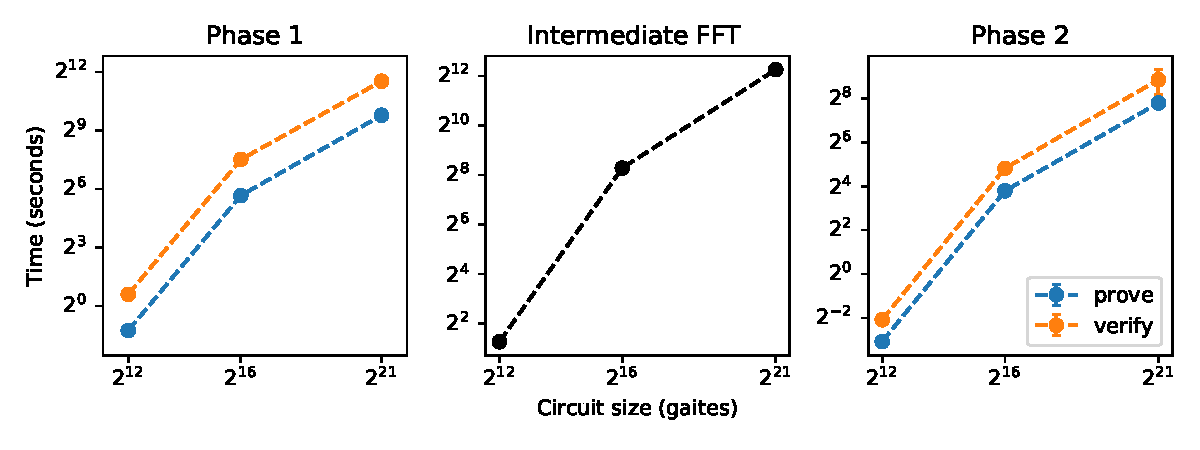
\includegraphics[width=\textwidth]{figure}
\centering
\caption{Performance of MMORPG protocol phases.  Averages taken over 5 iteration. Costs for phase 1 and 2 given for both prove and verification time. Individual participants need not run the verification function. Proving times take less than 16 minutes for all circuit sizes. Verification takes less then 55 minutes. We stress that verification is not run by individual users, it is done by the coordinator and anyone who wishes to verify the transcript of the protocol after completion.}
\label{fig:perf}
\end{figure*}
\paragraph{Computation:}

For $j\in \players$,
$P_j$ outputs
\begin{enumerate}
 \item \enc1{\delta_j}.
 \item$ y_{\delta,j}\defeq \pok{\delta_j}{\transcript_{2,j-1}}$.

  \item $\acc{\delta}{j}\defeq \acc{\delta}{j-1}/\delta_j$.
 \item For each $i\in [\ell+1..m]$, $\acc{K_i}{j}\defeq (\acc{K_i}{j-1})/\delta_j$.
 \item For each $i\in [0..n-2]$, $\acc{H_i}{j}\defeq (\acc{H_i}{j-1})/\delta_j$.
\end{enumerate}
In the end, we define
Let $J-1$ be the time-slot where $P_\numplayers$ sends their message.

\noindent
Let $\delta' \defeq \RB(J,1)$.
We define
\begin{enumerate}
\item $\enc0{\delta} \defeq \acc{\delta}{\numplayers}/\delta'$.
\item $\enc1{K_i}\defeq\acc{K_i}{\numplayers}/\delta'$.

\item $\enc1{H_i}\defeq \acc{H_i}{\numplayers}/\delta'$.

\end{enumerate}

\paragraph{Verification:}
The protocol verifier computes for each $j\in \players$
\[ r_{\delta,j}\defeq \RO(\enc1{\delta_j},\transcript_{2,j-1}),\]
and for each $j\in \players$ checks that
\begin{enumerate}
  \item \checkpok{\enc1{\delta_j}}{\transcript_{2,j-1}}{y_{\delta,j}}.
  \item For $j\in \players$, \consistent{\acc{\delta}{j-1}}{\acc{\delta}{j}}{(r_{\delta,j},y_{\delta,j})}.
 \item For each $i\in [\ell+1..m]$, $j\in \players$, \consistent{\acc{K_i}{j}}{\acc{K_i}{j-1}}{\enc0{\delta_j}}.
 \item For each $i\in [0..n-2]$, $j\in \players$, \consistent{\acc{H_i}{j}}{\acc{H_i}{j-1}}{\enc0{\delta_j}}.
\end{enumerate}

\section{BLS12-381}

The most common pairing-friendly elliptic curve construction used in {\snark} software is a Barreto-Naehrig~\cite{BN} (BN) construction with a 254-bit base field and group order, as designed in \cite{cryptoeprint:2013:507}. That construction equipts $\F$ with a large $2^n$ root of unity for efficient polynomial evaluation. Although the construction originally targeted the 128-bit security level, recent optimizations to the Number Field Sieve algorithm \cite{NFSOptimization} have reduced its concrete security.

Subsequent analysis \cite{cryptoeprint:2016:1102} recommended that BN curves and Barreto-Lynn-Scott (BLS) curves \cite{cryptoeprint:2002:088} with embedding degree $k = 12$ have approximately 384-bit base fields in order to target 128-bit security. BN curves are thus not ideal for our purposes, as these larger base fields are accompanied by similarly larger group orders, which substantially increases the cost of multi-exponentiation and fast-fourier transforms and harms the usability of protocols that use $\F$ to encode keying material. BLS12 curves with 384-bit base fields, in contrast, give rise to 256-bit group orders, making them ideal for use with {\snarks}. In more conservative contexts, the larger constructions proposed in \cite{cryptoeprint:2017:334} are recommended.

BLS curves with $k = 12$ are parameterized by an integer $x$. The existing BN curve has $2^{28} | p - 1$ to ensure a $2^{28}$ root of unity is available. We target the same by ensuring that $2^{14} | x$. We target prime $p$ of less than $2^{255}$ in order to accomodate efficient approximation algorithms and reductions. We desire efficient extension field towers and twisting isomorphisms, following recommendations from \cite{cryptoeprint:2012:232}. In addition, we desire $x$ of small Hamming weight for optimal pairing efficiency.

The largest construction with smallest Hamming weight that meets our requirements is $x = -2^{63} - 2^{62} - 2^{60} - 2^{57} - 2^{48} - 2^{16}$, which we name \textbf{BLS12-381}. This curve exists within a subfamily of curves, as in \cite{cryptoeprint:2011:465}, which have immediately determined curve parameters. We provide an implementation of this curve in Rust. \cite{pairinglibrary}


\newcommand{\circuitsmall}{$2^{10}$}
\newcommand{\circuitmedium}{$2^{17}$}
\newcommand{\circuitlarge}{$2^{21}$}
\section{Implementation and Experiments}
\label{sec:perf}
In this section, we evaluate our implementation of MMORPG. Our implementation of both MMORPG and the pairing library is in Rust. All benchmarks for phase 1 and 2  were done on a \texttt{Intel(R) Core(TM) i7-3770S CPU @ 3.10GHz} with 32GB of RAM running Arch Linux.


Because the performance of our protocol is independent of the number of participants, our experimental setup is exceedingly simple.  We need only measure the performance of a single user in each phase. 

The statements proven by a {\snarks} are represented by an arithmetic circuit. The size of the circuit, in terms of multiplication gates,  corresponds to the complexity of the statement that is proven. Our experimental setup consists of running MMORPG  for three different circuit sizes {\circuitsmall},{\circuitmedium},{\circuitlarge.} gates and measuring runtime and bandwidth.  {\circuitlarge} is the size of  the largest circuit publicly generated using\cite{BGG17} and corresponds to approximately 60 SHA256 invocations.  {\circuitmedium} corresponds to the size of the proposal for the next generation of zcash\cite{sapling} and {\circuitsmall} is a very small circuit. Performance numbers are given in \cref{fig:perf}. Bandwidth numbers for each phase and selected circuit sizes are given in \cref{tab:bandwidth}.

\begin{table}[h]
\centering
\caption{Bandwidth used in each phase}
\label{tab:bandwidth}
\begin{adjustbox}{width=\linewidth}
\centering
\begin{tabular}{l|l|l|l|l|}
\cline{2-5}
                                           & \multicolumn{4}{c|}{protocol phase}                         \\ \cline{2-5} 
                                           & \multicolumn{2}{c|}{phase 1} & \multicolumn{2}{c|}{phase 2} \\ \hline
\multicolumn{1}{|c|}{circuit size}         & down          & up           & down          & up           \\ \hline
\multicolumn{1}{|l|}{2\textasciicircum 11} & 0.59 MB        & 0.29  MB      & 0.19 MB        & 0.09 MB       \\ \hline
\multicolumn{1}{|l|}{2\textasciicircum 12} & 75.5 MB        & 37.75 MB       & 25.17 MB        & 12.58 MB        \\ \hline
\multicolumn{1}{|l|}{2\textasciicircum 15} & 1.13 GB        & 0.56 GB       & 0.37 GB        & 0.19 GB       \\ \hline
\end{tabular}
\end{adjustbox}
\end{table}


For completeness we also profile the interphase computation by the coordinator. This step is costly. We stress that this computation does not involve secret data and need only be done one once. In practice a large AWS EC2 instance would be rented for this computation.


These results show that the protocol is  practical. A user need only spend 15 minutes doing a computation and after that need no longer participate. This means participation requires low investment and does not require the user to maintain a heightened state of security for hours or days.  Moreover, it is a \imm{FIXME SEAN} X improvement on the per user computation time of the real world execution of\cite{BGG17}. We stress that this is not a result of moving to the new curve, since that curve has a higher computational complexity and would, for identical implementations,be slower than the \texttt{BN128} used in\cite{BGG17}. Instead it is the result of both avoiding the need for pre-commitment phase and resulting idle time and of protocol and software optimizations that improve the actual computation time.




 \section*{Acknowledgements}
 We thank Paulo Barreto for helpful feedback about the BLS12-381 elliptic curve. We thank Daniel Benarroch and Daira Hopwood for helpful comments. We thank the anonymous reviewers of S\&P 2018 for their comments.


\bibliographystyle{plain}
\bibliography{paper}
\end{document}

